%% ============================================================
%%  Adaptive Neural Control for Mars Rover Wheel
%%  Entrapment Recovery in Granular Terrain
%%  Beamer Presentation: University of Dhaka, RME 4100
%%  Authors: Meraj Hossain Promit & Chandak Chakma
%%  2026: Light Theme Edition
%% ============================================================

\documentclass[aspectratio=169, 10pt]{beamer}

%% ── Packages ─────────────────────────────────────────────────
\usepackage[utf8]{inputenc}
\usepackage[T1]{fontenc}
\usepackage{lmodern}
\usepackage{microtype}
\usepackage{amsmath, amssymb}
\usepackage{bm}
\usepackage{booktabs}
\usepackage{colortbl}
\usepackage{tabularx}
\usepackage{multirow}
\usepackage{tikz}
\usetikzlibrary{arrows.meta, shapes.geometric, positioning,
                decorations.pathreplacing, fadings, backgrounds,
                calc, fit, matrix}
\usepackage{pgfplots}
\pgfplotsset{compat=1.18}
\usepackage{fontawesome5}
\usepackage{xcolor}
\usepackage{graphicx}
\graphicspath{{../figures/}{../../experiments/regolith_recovery/plots/}{../../experiments/sim2sim/figs/}}
\usepackage{array}
\usepackage{ragged2e}
\usepackage{etoolbox}
\usepackage[most]{tcolorbox}
\usepackage{enumitem}
\usepackage{multimedia}  % Beamer built-in video embedding (\movie command)

%% ── Report diagram colors (ported from project_report.tex) ──
\definecolor{marsred}{RGB}{150,40,20}
\definecolor{deepblue}{RGB}{40,60,100}
\definecolor{boxgray}{RGB}{248,248,248}
\definecolor{headerblue}{RGB}{50,80,130}
\definecolor{accentorange}{RGB}{200,100,30}
\definecolor{softgreen}{RGB}{60,140,60}
\definecolor{softpurple}{RGB}{100,60,150}
\definecolor{lightblue}{RGB}{220,235,250}
\definecolor{lightorange}{RGB}{255,235,210}
\definecolor{lightred}{RGB}{255,220,220}
\definecolor{lightgreen}{RGB}{220,245,220}

%% ── Color Palette (Light Background + Dark Text) ────────────
\definecolor{SpaceBlack}{HTML}{FFFFFF} % Main background
\definecolor{MarsRust}{HTML}{C1440E}
\definecolor{MarsLight}{HTML}{B33A0A}  % Slightly darker for white bg
\definecolor{CosmicBlue}{HTML}{E9ECEF} % Light gray for cards/headers
\definecolor{StarWhite}{HTML}{111111}  % Main text (near-black)
\definecolor{NebulaPurple}{HTML}{4A3F8C}
\definecolor{ArcticTeal}{HTML}{00897B} % Darker teal for contrast
\definecolor{SandGold}{HTML}{A67C00}   % Darker gold
\definecolor{SlideGray}{HTML}{F8F9FA}  % Subtle alternating row
\definecolor{TextLight}{HTML}{2D3748}  % Body text
\definecolor{AccentGreen}{HTML}{2E7D32} % Darker green
\definecolor{WarnOrange}{HTML}{E65100}
\definecolor{MutedBlue}{HTML}{455A64}  % Dark slate for secondary text
\definecolor{CardBg}{HTML}{F4F6F9}     % Card background
\definecolor{DimText}{HTML}{6C757D}    % Muted/secondary text
\definecolor{Green}{HTML}{28A745}
\definecolor{BorderGray}{HTML}{DEE2E6} % For box borders

%% ── Beamer Theme Customization ───────────────────────────────
\usetheme{default}
\usecolortheme{default}
\setbeamertemplate{navigation symbols}{}
\setbeamertemplate{itemize items}{\color{MarsRust}\faChevronRight}
\setbeamertemplate{itemize subitems}{\color{ArcticTeal}\faAngleRight}
\setbeamertemplate{enumerate items}[default]

\setbeamercolor{background canvas}{bg=SpaceBlack}
\setbeamercolor{normal text}{fg=StarWhite}
\setbeamercolor{frametitle}{fg=StarWhite}
\setbeamercolor{title}{fg=StarWhite}
\setbeamercolor{subtitle}{fg=TextLight}
\setbeamercolor{author}{fg=MutedBlue}
\setbeamercolor{date}{fg=DimText}
\setbeamercolor{itemize item}{fg=MarsRust}
\setbeamercolor{itemize subitem}{fg=ArcticTeal}
\setbeamercolor{block title}{bg=CosmicBlue, fg=StarWhite}
\setbeamercolor{block body}{bg=CardBg, fg=TextLight}

%% Fonts
\setbeamerfont{frametitle}{size=\large, series=\bfseries}
\setbeamerfont{title}{size=\LARGE, series=\bfseries}
\setbeamerfont{subtitle}{size=\normalsize, series=\mdseries}

%% ── tcolorbox styles ─────────────────────────────────────────
\tcbset{
  mycard/.style={
    enhanced, colback=CardBg, colframe=BorderGray,
    boxrule=0.5pt, arc=4pt, left=4pt, right=4pt,
    top=3pt, bottom=3pt, fonttitle=\bfseries\small,
    coltitle=MarsLight
  },
  statbox/.style={
    enhanced, colback=CardBg, colframe=BorderGray,
    boxrule=1pt, arc=6pt, halign=center, valign=center,
    left=4pt, right=4pt, top=4pt, bottom=4pt
  },
  highlight/.style={
    enhanced, colback=MarsRust!10, colframe=MarsRust!40,
    boxrule=0.8pt, arc=3pt, left=5pt, right=5pt,
    top=2pt, bottom=2pt
  },
  greenbox/.style={
    enhanced, colback=AccentGreen!10, colframe=AccentGreen!60,
    boxrule=0.8pt, arc=3pt, left=5pt, right=5pt,
    top=2pt, bottom=2pt
  }
}

%% ── Helpers ──────────────────────────────────────────────────
\newcommand{\BIG}[1]{{\fontsize{28}{32}\selectfont\bfseries\color{MarsLight}#1}}
\newcommand{\MED}[1]{{\fontsize{18}{22}\selectfont\bfseries\color{ArcticTeal}#1}}
\newcommand{\keyword}[1]{\textbf{\color{MarsLight}#1}}
\newcommand{\teal}[1]{{\color{ArcticTeal}#1}}
\newcommand{\rust}[1]{{\color{MarsRust}#1}}
\newcommand{\gold}[1]{{\color{SandGold}#1}}
\newcommand{\tick}{\textcolor{AccentGreen}{\faCheckCircle}}
\newcommand{\arrow}{\textcolor{MarsRust}{\faArrowRight}\;}
\newcommand{\warn}{\textcolor{WarnOrange}{\faExclamationTriangle}\;}

%% Wider content area helper
\newcommand{\fullrow}[1]{\noindent\hspace{-0.25cm}#1}

%% ── Document ─────────────────────────────────────────────────
\begin{document}

%% ── SLIDE 1: TITLE ───────────────────────────────────────────
{
\setbeamertemplate{footline}{}
\setbeamertemplate{frametitle}{}
\begin{frame}[plain]
\begin{tikzpicture}[remember picture, overlay]
  %% ── Background & Decorations ─────────────────────────────
  \fill[SpaceBlack] (current page.south west) rectangle (current page.north east);
  \fill[CosmicBlue!40, opacity=0.5] (current page.south west) -- ++(16.9,0) -- ++(0,4) -- cycle;

  %% Stars
  \foreach \x/\y in {1/8, 3/7.2, 5/8.5, 7/7.8, 9/8.2, 11/7.5, 13/8.1, 15/7.4,
                      2/6, 4/5.8, 6/6.3, 8/5.5, 10/6.1, 12/5.7, 14/6.4,
                      0.5/4, 2.5/3.8, 16/8.3, 16.5/6.5} {
    \fill[DimText, opacity=0.35] (\x,\y) circle (0.5pt);
  }

  %% Mars Circle
  \fill[MarsRust, opacity=0.08] (14.5, 4.75) circle (2.8cm);
  \fill[MarsRust, opacity=0.05] (14.5, 4.75) circle (3.5cm);
  \draw[MarsRust, opacity=0.2, line width=0.5pt] (14.5, 4.75) circle (3.1cm);

  %% Red Accent Bar
  \fill[MarsRust] (0, 0) rectangle (0.18, 9.6);

  %% ── TEXT ELEMENTS ──

  %% 1. University Header
  \node[anchor=north west, text=DimText, font=\tiny\itshape]
    at ([shift={(1.5cm,-0.6cm)}]current page.north west)
    {University of Dhaka \quad|\quad Dept.\ of Robotics \& Mechatronics Engineering \quad|\quad RME 4100: Project 2026};

  %% 2. Main Title
  \node[anchor=north west, text=StarWhite, font=\bfseries\LARGE,
        align=left, text width=13cm]
    at ([shift={(1.5cm,-1.5cm)}]current page.north west)
    {Adaptive Neural Control for\vspace{0.4em}\\
     \textcolor{MarsLight}{Mars Rover Wheel Entrapment}\vspace{0.4em}\\
     Recovery in Granular Terrain};

  %% 3. Divider Line
  \draw[MarsRust!50, line width=0.8pt] ([shift={(0.5cm,-4.5cm)}]current page.north west) -- ++(13cm,0);

  %% 4. Authors
  \node[anchor=north west, text=TextLight, font=\normalsize\bfseries]
    at ([shift={(0.5cm,-5.2cm)}]current page.north west)
    {Meraj Hossain Promit \quad \& \quad Chandak Chakma};

  %% 5. Supervisors — centred, side by side, close together
  \node[anchor=north, text=TextLight, font=\scriptsize, align=center,
        text width=5.5cm]
    at ([shift={(-2.2cm,-6.5cm)}]current page.north)
    {\textbf{Supervisor}\\[1pt]
     \textcolor{ArcticTeal}{Md.\ Jubair Ahmed Sourav}\\
     Lecturer, Dept.\ of Robotics \&\\Mechatronics Engineering\\
     University of Dhaka};

  \node[anchor=north, text=TextLight, font=\scriptsize, align=center,
        text width=5.5cm]
    at ([shift={(2.2cm,-6.5cm)}]current page.north)
    {\textbf{Co-Supervisor}\\[1pt]
     \textcolor{ArcticTeal}{Dr.\ Sejuti Rahman}\\
     Associate Professor, Dept.\ of Robotics \&\\Mechatronics Engineering\\
     University of Dhaka};

  %% 6. Martian terrain silhouette — anchored to the very bottom edge
  \begin{scope}[shift={(current page.south west)}, opacity=0.22]
    %% back dune layer (darker)
    \fill[MarsRust!80]
      (0,0) -- (0,0.75)
      .. controls (1.5,1.3) and (2.8,0.5) .. (4.5,0.9)
      .. controls (6.0,1.3) and (7.2,0.45) .. (9.0,0.85)
      .. controls (10.5,1.25) and (11.8,0.5) .. (13.5,0.95)
      .. controls (14.8,1.3) and (15.8,0.6) .. (16.9,1.0)
      -- (16.9,0) -- cycle;
    %% front dune layer (lighter, lower)
    \fill[MarsRust!50]
      (0,0) -- (0,0.45)
      .. controls (2.2,0.85) and (4.0,0.2) .. (6.0,0.55)
      .. controls (7.8,0.9) and (9.5,0.2) .. (11.5,0.5)
      .. controls (13.0,0.8) and (14.8,0.25) .. (16.9,0.6)
      -- (16.9,0) -- cycle;
  \end{scope}

  %% Wheel tracks — just above the terrain surface
  \begin{scope}[shift={(current page.south west)}, opacity=0.15,
                MarsRust!60, line width=0.55pt, dashed]
    \draw (0.5,0.65) .. controls (4.5,0.95) and (9.0,0.6) .. (15.5,0.8);
    \draw (0.5,0.45) .. controls (4.5,0.75) and (9.0,0.4) .. (15.5,0.6);
  \end{scope}

  %% Crater rim arc — bottom right corner
  \begin{scope}[shift={(current page.south east)}, opacity=0.12]
    \draw[MarsRust!70, line width=1.0pt]
      (-1.0,0) arc[start angle=160, end angle=20, radius=2.8cm];
  \end{scope}

  %% 7. DU Logo (top right)
  \node[anchor=north east]
    at ([shift={(-0.4cm,-0.3cm)}]current page.north east)
    {
\includegraphics[height=1.4cm]{du_logo}};

  %% 8. Year
  \node[anchor=south east, text=DimText, font=\tiny]
    at ([shift={(-0.5cm,0.5cm)}]current page.south east) {19 April, 2026};

\end{tikzpicture}
\end{frame}
}

%% ── SLIDE 2: MOTIVATION ──────────────────────────────────────
\begin{frame}{The Problem That Started It All}
\begin{columns}[T]
  \column{0.52\textwidth}
   \vspace{-1.5em}
  \begin{tcolorbox}[mycard, title={\faRocket\; The Spirit Rover Incident: May 2009}]
    \small
    \begin{itemize}[leftmargin=1em, itemsep=3pt]
      \item[\rust{\faCircle[regular]}] After \keyword{5 years} of exploration, Spirit drove into soft
        sulfate-rich regolith at \textit{``Troy''}
      \item[\rust{\faCircle[regular]}] \keyword{8 months} of Earth-based recovery attempts, all failed
      \item[\rust{\faCircle[regular]}] One-way signal latency: \keyword{4–24 minutes}
      \item[\rust{\faCircle[regular]}] No autonomous escape capability onboard
      \item[\rust{\faCircle[regular]}] Mission permanently ended; rover never moved again
    \end{itemize}
     \vspace{-1.4em}
    \medskip
    \begin{tcolorbox}[highlight]
      \centering\small\textit{``What if the rover could have \textbf{saved itself}?''}
    \end{tcolorbox}
  \end{tcolorbox}

  \vspace{-1.1em}
  \begin{tcolorbox}[mycard, title={\faExclamationCircle\; Why Autonomous Recovery?}]
    \scriptsize
    \begin{tabular}{@{}cl@{}}
      \teal{\faWifi} & Real-time teleoperation: \rust{impossible} at 4–24 min latency \\[2pt]
      \teal{\faCog}  & Rocker-bogie suspension: complex sinkage dynamics \\[2pt]
      \teal{\faGlobe} & Martian regolith: highly unpredictable granular behaviour \\[2pt]
      \teal{\faClock} & Extended missions encounter unanticipated terrain types \\
    \end{tabular}
  \end{tcolorbox}

  \column{0.46\textwidth}
  %% Spirit timeline
  \begin{tikzpicture}[scale=0.82]
    \draw[MarsRust!30, line width=1.5pt] (0,5.8) -- (0,0);
    \foreach \y/\yr/\ev/\col in {
        5.5/{Jan 2004}/{Spirit Lands on Mars}/{AccentGreen},
        4.4/{Apr 2009}/{5 Years Successful Exploration}/{ArcticTeal},
        3.3/{May 2009}/{\textbf{Entrapped at ``Troy''}}/{MarsRust},
        2.2/{Jun–Dec 2009}/{8-Month Rescue Attempt}/{WarnOrange},
        1.1/{Jan 2010}/{Stationary Science Mode}/{SandGold},
        0.0/{May 2011}/{Contact Lost: Mission Ended}/{MutedBlue}
    }{
      \fill[\col] (-0.07,\y) circle (3.5pt);
      \draw[\col, line width=0.6pt] (0.07,\y) -- (0.5,\y);
      \node[anchor=west, text=DimText, font=\tiny] at (0.55, \y+0.2) {\yr};
      \node[anchor=west, text=TextLight, font=\scriptsize, text width=4.5cm] at (0.55, \y-0.12) {\ev};
    }
  \end{tikzpicture}

  \vspace{0.4em}
  \begin{tcolorbox}[statbox, title={}]
    \centering
    {\color{MarsLight}\bfseries\Large 150M km}\\
    {\color{DimText}\scriptsize Earth–Mars distance during entrapment}
  \end{tcolorbox}
\end{columns}
\end{frame}

%% ── SLIDE 2b: SPIRIT TIMELINE ────────────────────────────────
\begin{frame}{The Spirit Rover Entrapment: A 7-Year Timeline}
\vspace{0.2em}
\begin{tcolorbox}[mycard, title={\faClock\; Chronology of the Spirit Entrapment Incident (2004–2011)}]
\centering
\resizebox{\linewidth}{!}{%
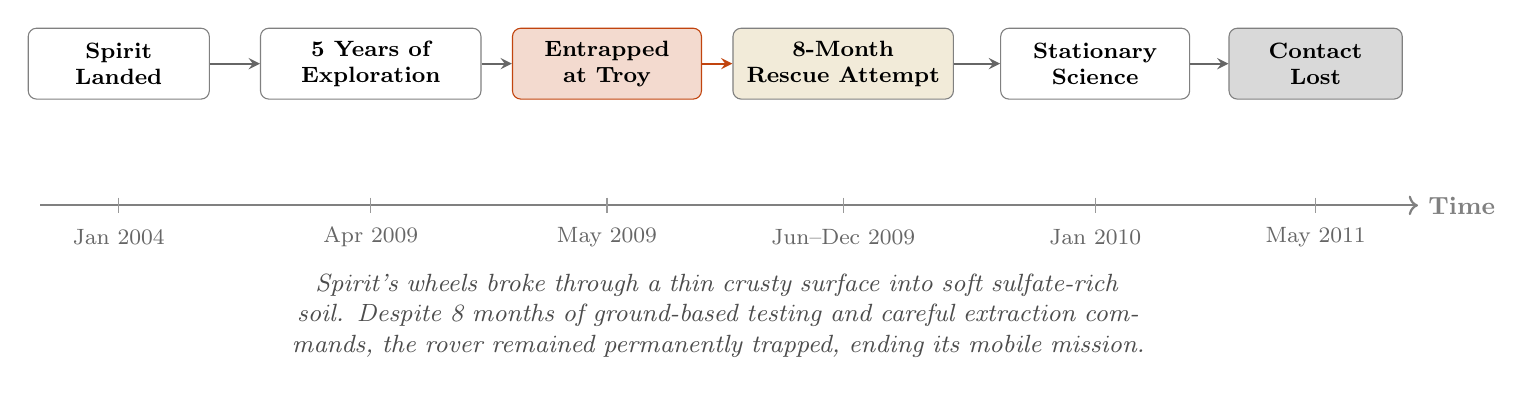
\begin{tikzpicture}[
    box/.style={rectangle, rounded corners=3pt, draw=black!50, fill=white,
                minimum height=0.9cm, align=center, font=\footnotesize\bfseries},
    arrow/.style={->, >=stealth, thick, color=black!60}
]
    \node[box, minimum width=2.3cm] (b1) at (0,0) {Spirit\\Landed};
    \node[box, minimum width=2.8cm] (b2) at (3.2,0) {5 Years of\\Exploration};
    \node[box, minimum width=2.4cm, fill=MarsRust!20, draw=MarsRust] (b3) at (6.2,0) {Entrapped\\at Troy};
    \node[box, minimum width=2.8cm, fill=SandGold!15] (b4) at (9.2,0) {8-Month\\Rescue Attempt};
    \node[box, minimum width=2.4cm] (b5) at (12.4,0) {Stationary\\Science};
    \node[box, minimum width=2.2cm, fill=black!15] (b6) at (15.2,0) {Contact\\Lost};
    \draw[arrow] (b1) -- (b2);
    \draw[arrow] (b2) -- (b3);
    \draw[arrow, color=MarsRust] (b3) -- (b4);
    \draw[arrow] (b4) -- (b5);
    \draw[arrow] (b5) -- (b6);
    \draw[->, thick, color=black!50] (-1,-1.8) -- (16.5,-1.8) node[right, font=\small\bfseries] {Time};
    \foreach \x/\lbl in {0/Jan 2004, 3.2/Apr 2009, 6.2/May 2009,
                          9.2/Jun--Dec 2009, 12.4/Jan 2010, 15.2/May 2011} {
        \draw[black!40] (\x,-1.7) -- (\x,-1.9);
        \node[font=\footnotesize, text=black!60] at (\x,-2.2) {\lbl};
    }
    \node[text width=15cm, align=center, font=\small\itshape, text=black!70] at (7.6,-3.2) {
        Spirit's wheels broke through a thin crusty surface into soft sulfate-rich soil.
        Despite 8 months of ground-based testing and careful extraction commands,
        the rover remained permanently trapped, ending its mobile mission.
    };
\end{tikzpicture}%
}
\end{tcolorbox}
\vspace{0.3em}
\begin{tcolorbox}[highlight]
  \scriptsize\centering
  \textbf{Key lesson:} Spirit had \emph{no onboard capability} to detect or respond to entrapment autonomously.
  All recovery attempts were commanded from Earth with 8–40 min round-trip delay.
  \textbf{Our work builds the autonomy Spirit never had.}
\end{tcolorbox}
\end{frame}

%% ── SLIDE 3: OBJECTIVES ──────────────────────────────────────
\begin{frame}{Research Objectives}
\vspace{0.2em}
\begin{columns}[T]
\column{0.5\textwidth}

\begin{tcolorbox}[mycard, title={\faFlask\; Obj 1: Realistic Simulation}]
  \scriptsize
  Couple \keyword{Newton MPM} granular physics with \keyword{Isaac Lab}
  rigid-body solver under \teal{Martian gravity (3.72 m/s²)}
\end{tcolorbox}
\vspace{0.25em}

\begin{tcolorbox}[mycard, title={\faRadiation\; Obj 2: Entrapment Detection}]
  \scriptsize
  Dual-sensor scheme: \keyword{slip-ratio monitoring} +
  \keyword{drive-torque anomaly}: no GPS, no external sensing
\end{tcolorbox}
\vspace{0.25em}

\begin{tcolorbox}[mycard, title={\faBrain\; Obj 3: Recovery Policy}]
  \scriptsize
  Recurrent RL policy (\keyword{PPO + GRU}) discovering rocking,
  steering pivots, and differential drive for varying sinkage
\end{tcolorbox}

\column{0.48\textwidth}

\begin{tcolorbox}[mycard, title={\faGraduationCap\; Obj 4: Curriculum Learning}]
  \scriptsize
  Progressive sinkage: \keyword{15 cm → 28 cm} across 64 parallel
  environments; enables generalisation across terrain conditions
\end{tcolorbox}
\vspace{0.25em}

\begin{tcolorbox}[mycard, title={\faSyncAlt\; Obj 5: Sim-to-Sim \& Sim-to-Real}]
  \scriptsize
  \textbf{Primary:} Cross-simulator validation (MuJoCo / Gazebo),
  sloped beds ±15°, variable soil density\\[3pt]
  \textbf{Secondary:} ONNX export → \keyword{Raspberry Pi 5} at 10 Hz
\end{tcolorbox}
\vspace{0.25em}

\begin{tcolorbox}[greenbox]
  \scriptsize\centering
  \tick\; \textbf{Novel contribution:} First DRL escape system for a
  6-wheel rocker-bogie rover in physics-accurate granular simulation
\end{tcolorbox}

\end{columns}
\end{frame}

%% ── SLIDE 4: RELATED WORK ────────────────────────────────────
\begin{frame}{Related Work \& Research Gaps}
\vspace{0.1em}
{\tiny\setlength{\tabcolsep}{4pt}
\begin{tabularx}{\textwidth}{@{}l l X c c c@{}}
  \toprule
  \rowcolor{MarsRust!10}
  \color{StarWhite}\textbf{Work} &
  \color{StarWhite}\textbf{Robot} &
  \color{StarWhite}\textbf{Key Limitation} &
  \color{StarWhite}\textbf{Terrain} &
  \color{StarWhite}\textbf{Gravity} &
  \color{StarWhite}\textbf{Escape\%} \\
  \midrule
  \rowcolor{CardBg}
  Bi \& Ding (2026) & 4-wheel SSMR & No granular physics; needs expert demos & Rigid & Earth & 90\% \\
  \rowcolor{SlideGray}
  Mortensen \& Bøgh (2024) & AAU 6-wheel & Navigation only; no entrapment/recovery task & Rigid & Mars & N/A \\
  \rowcolor{CardBg}
  Inotsume (2020) & 6-wheel & Detection only; no recovery policy & Bekker & Mars & N/A \\
  \rowcolor{SlideGray}
  Jain (2019) & 6-wheel & Discrete action space; approx.\ terrain & Approx. & Mars & N/A \\
  \rowcolor{CardBg}
  Fankhauser (2018) & ANYmal & Legged robot; different failure mode & Rigid & Earth & N/A \\
  \midrule
  \rowcolor{MarsRust!15}
  \textbf{Ours} & \textbf{6-wheel RB} & \textbf{sim2sim validation in progress} &
    \teal{\textbf{MPM}} & \teal{\textbf{Mars}} & \textbf{$\sim$87\%} \\
  \bottomrule
\end{tabularx}
}

\vspace{0.2em}
\begin{tcolorbox}[mycard, title={\faRobot\; Key Dependency: RLRoverLab (Mortensen \& Bøgh, ISPaRo 2024)}]
  \tiny
  Open-source RL suite on NVIDIA ORBIT/Isaac Sim. Provides the \keyword{AAU Rover Complex} USD asset
  and pre-trained \keyword{navigation policies} (our Navigation Brain).
  \textbf{Gap we fill:} rigid terrain only; no granular physics, no entrapment task.
  We add Newton MPM coupling for regolith sinkage and recovery.
\end{tcolorbox}

\vspace{0.2em}
\begin{columns}[T]
\column{0.32\textwidth}
\begin{tcolorbox}[mycard, title={\faExclamationCircle\; Gap 1}]
  \tiny No prior work: 6-wheel rocker-bogie + MPM granular + DRL
\end{tcolorbox}
\column{0.32\textwidth}
\begin{tcolorbox}[mycard, title={\faExclamationCircle\; Gap 2}]
  \tiny Granular progressive sinkage unstudied in DRL context
\end{tcolorbox}
\column{0.32\textwidth}
\begin{tcolorbox}[mycard, title={\faExclamationCircle\; Gap 3}]
  \tiny Mars gravity + independent 10D per-wheel control unexplored
\end{tcolorbox}
\end{columns}
\end{frame}

%% ── SLIDE 4b: COMPARISON WITH BI & DING ─────────────────────
\begin{frame}{Comparison with State-of-the-Art: Bi \& Ding (2026)}
\vspace{0.1em}
\begin{columns}[T]
\column{0.58\textwidth}
{\scriptsize\setlength{\tabcolsep}{4pt}
\begin{tabularx}{\linewidth}{@{}l X X@{}}
  \toprule
  \rowcolor{MarsRust!8}
  \color{StarWhite}\textbf{Aspect} &
  \color{MutedBlue}\textbf{Bi \& Ding (2026)} &
  \color{MarsLight}\textbf{Ours} \\
  \midrule
  \rowcolor{CardBg}
  Robot & 4-wheel SSMR & \teal{6-wheel RB} \\
  \rowcolor{SlideGray}
  Terrain & Rigid (Unity) & \teal{MPM (Newton)} \\
  \rowcolor{CardBg}
  Gravity & Earth & \teal{Mars} \\
  \rowcolor{SlideGray}
  Obs & 30D & 29D \\
  \rowcolor{CardBg}
  Action & 2D & \teal{10D} \\
  \rowcolor{SlideGray}
  Policy & PPO+LSTM & PPO+GRU \\
  \rowcolor{CardBg}
  Steps & 4M & 200K \\
  \rowcolor{SlideGray}
  Reward & GAIL+expert & \teal{Handcrafted} \\
  \rowcolor{CardBg}
  Escape & \textbf{90\%} & \teal{$\sim$87\%} \\
  \rowcolor{SlideGray}
  Real-world & \teal{Yes} & Planned \\
  \bottomrule
\end{tabularx}
}

\vspace{0.3em}
\begin{tcolorbox}[highlight]
  \tiny
  \textbf{\faExclamationTriangle\; Their edge:} 20$\times$ more training, real-world validated, GAIL+expert demos
\end{tcolorbox}
\vspace{0.2em}
\begin{tcolorbox}[greenbox]
  \tiny
  \textbf{\faCheckCircle\; Our edge:} physics-accurate MPM soil, Mars gravity, 5$\times$ richer action space, no expert data
\end{tcolorbox}

\column{0.40\textwidth}
\begin{tcolorbox}[mycard, title={\faMicrochip\; Why GRU not LSTM?}]
  \tiny
  \textbf{GRU advantages:}
  \begin{itemize}[leftmargin=1em, itemsep=2pt]
    \item 2 gates vs.\ 3 in LSTM; $\sim$30\% fewer params
    \item Faster on RPi5 ($<$5\,ms vs.\ $\sim$7\,ms)
    \item No cell state; simpler BPTT
  \end{itemize}
  \vspace{3pt}
  \textbf{LSTM not needed:}
  \begin{itemize}[leftmargin=1em, itemsep=2pt]
    \item Episodes 200--600 steps, seq=16; no very long dependencies
    \item GRU matches LSTM for sequences $\le$5\,s
    \item PPO clipping already stabilises gradients
  \end{itemize}
\end{tcolorbox}
\end{columns}
\end{frame}

%% ── SLIDE 5b: ESCAPE POLICY GENERATION (Fig 2) ───────────────
\begin{frame}{Escape Policy Generation: Training \& Deployment (Fig.~2)}
\vspace{-0.3em}
\centering
\resizebox{!}{0.80\textheight}{%
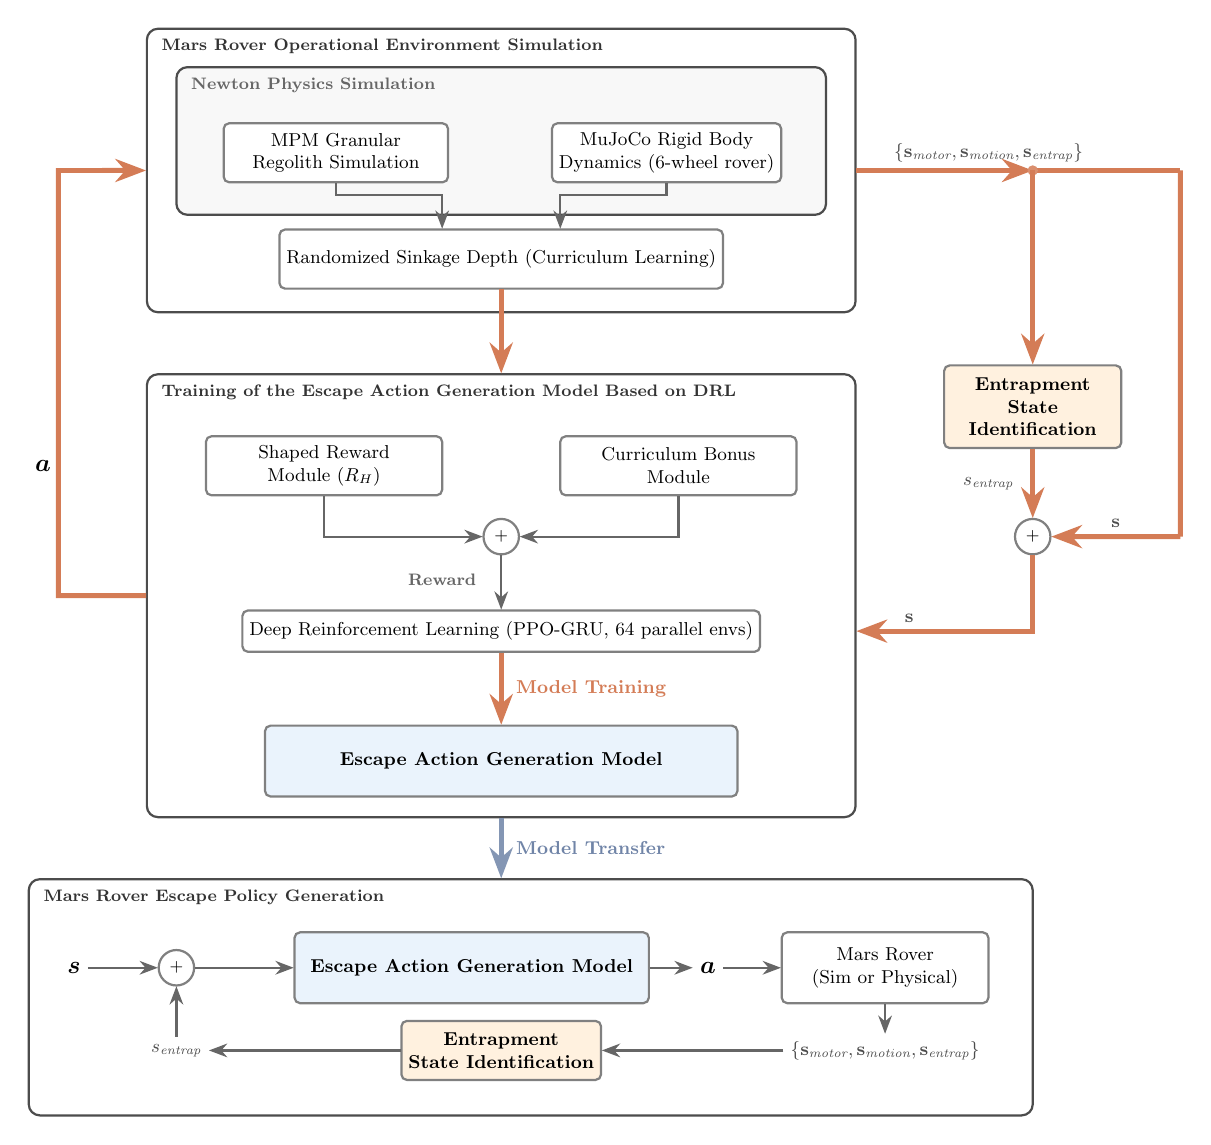
\begin{tikzpicture}[
    scale=0.75, transform shape,
    outerbox/.style={rectangle, draw=black!70, thick, rounded corners=4pt, inner sep=10pt},
    innerbox/.style={rectangle, draw=black!50, thick, fill=white,
                     minimum height=1cm, minimum width=3.8cm,
                     align=center, font=\small, rounded corners=2pt},
    orangebox/.style={innerbox, fill=lightorange!70, font=\small\bfseries},
    bluebox/.style={innerbox, fill=lightblue!60, font=\small\bfseries},
    redarrow/.style={-Stealth, line width=1.8pt, color=MarsRust!70},
    bluearrow/.style={-Stealth, line width=1.8pt, color=headerblue!60},
    arrow/.style={-Stealth, thick, color=black!60},
    circnode/.style={draw=black!50, circle, thick, minimum size=0.6cm,
                     inner sep=0pt, font=\footnotesize},
    every node/.style={font=\small}
]
\node[outerbox, fill=white, minimum width=12cm, minimum height=4.8cm] (simbox) at (0, 12.5) {};
\node[font=\footnotesize\bfseries, anchor=north west, text=black!80]
    at ([xshift=4pt, yshift=-2pt]simbox.north west)
    {Mars Rover Operational Environment Simulation};
\node[outerbox, fill=boxgray, minimum width=11cm, minimum height=2.5cm] (physbox) at (0, 13.0) {};
\node[font=\footnotesize\bfseries, anchor=north west, text=black!60]
    at ([xshift=4pt, yshift=-2pt]physbox.north west) {Newton Physics Simulation};
\node[innerbox] (mpm) at (-2.8, 12.8) {MPM Granular\\Regolith Simulation};
\node[innerbox] (rigid) at (2.8, 12.8) {MuJoCo Rigid Body\\Dynamics (6-wheel rover)};
\node[innerbox, minimum width=7cm] (terrain) at (0, 11.0) {Randomized Sinkage Depth (Curriculum Learning)};
\node[orangebox, minimum width=3cm, minimum height=1.4cm] (entrapid) at (9, 8.5) {\textbf{Entrapment}\\State\\Identification};
\node[outerbox, fill=white, minimum width=12cm, minimum height=7.5cm] (trainbox) at (0, 5.3) {};
\node[font=\footnotesize\bfseries, anchor=north west, text=black!80]
    at ([xshift=4pt, yshift=-2pt]trainbox.north west)
    {Training of the Escape Action Generation Model Based on DRL};
\node[innerbox, minimum width=4cm] (handrew) at (-3, 7.5) {Shaped Reward\\Module ($R_H$)};
\node[innerbox, minimum width=4cm] (curricrew) at (3, 7.5) {Curriculum Bonus\\Module};
\node[circnode] (plus) at (0, 6.3) {$+$};
\node[below=0.2cm of plus, xshift=-1.0cm, font=\footnotesize\bfseries, text=black!60] {Reward};
\node[innerbox, minimum width=8cm, minimum height=0.7cm] (drl) at (0, 4.7) {Deep Reinforcement Learning (PPO-GRU, 64 parallel envs)};
\node[circnode] (sconcat) at (9, 6.3) {$+$};
\node[font=\large\bfseries\itshape, anchor=east] (abig) at (-7.5, 7.5) {$\boldsymbol{a}$};
\node[bluebox, minimum width=8cm, minimum height=1.2cm] (escapemodel) at (0, 2.5) {\textbf{Escape Action Generation Model}};
\draw[arrow] (mpm.south) -- ++(0,-0.2) -| ([xshift=-1cm]terrain.north);
\draw[arrow] (rigid.south) -- ++(0,-0.2) -| ([xshift=1cm]terrain.north);
\draw[redarrow] (terrain.south) -- (trainbox.north);
\coordinate (split) at (9, 12.5);
\coordinate (hTip)  at (11.5, 12.5);
\draw[redarrow] (simbox.east) -- (split)
    node[pos=0.75, above, font=\small\itshape, text=black!70]
        {$\{\mathbf{s}_{\text{motor}}, \mathbf{s}_{\text{motion}}, \mathbf{s}_{\text{entrap}}\}$};
\draw[redarrow, -{}] (split) -- (hTip);
\fill[MarsRust!60] (split) circle (2.5pt);
\draw[redarrow] (split) -- (entrapid.north);
\draw[redarrow] (entrapid.south) -- (sconcat.north)
    node[midway, left=5pt, font=\small\itshape, text=black!70] {$s_{\text{entrap}}$};
\draw[redarrow, -{}] (hTip) -- (11.5, 6.3);
\draw[redarrow] (11.5, 6.3) -- (sconcat.east)
    node[midway, above, font=\small\itshape, text=black!70] {$\mathbf{s}$};
\draw[redarrow] (sconcat.south) -- (sconcat.south |- drl) -- (trainbox.east |- drl)
    node[pos=0.7, above, font=\small\itshape, text=black!70] {$\mathbf{s}$};
\draw[arrow] (handrew.south) |- (plus.west);
\draw[arrow] (curricrew.south) |- (plus.east);
\draw[arrow] (plus.south) -- (drl.north);
\draw[redarrow] (trainbox.west) -- (-7.5, 5.3) -- (-7.5, 12.5) -- (simbox.west);
\draw[redarrow] (drl.south) -- (escapemodel.north)
    node[midway, right=3pt, font=\small\bfseries, text=MarsRust!70] {Model Training};
\node[outerbox, fill=white, minimum width=17cm, minimum height=4cm] (deploybox) at (0.5, -1.5) {};
\node[font=\footnotesize\bfseries, anchor=north west, text=black!80]
    at ([xshift=4pt, yshift=-2pt]deploybox.north west)
    {Mars Rover Escape Policy Generation};
\node[circnode] (sconcat2) at (-5.5, -1.0) {$+$};
\node[font=\large\bfseries\itshape, anchor=east] (slbl2) at (-7.0, -1.0) {$\boldsymbol{s}$};
\node[bluebox, minimum width=6cm, minimum height=1.2cm] (escapemodel2) at (-0.5, -1.0) {\textbf{Escape Action Generation Model}};
\node[font=\large\bfseries\itshape] (abig2) at (3.5, -1.0) {$\boldsymbol{a}$};
\node[innerbox, minimum width=3.5cm, minimum height=1.2cm] (physical) at (6.5, -1.0) {Mars Rover\\(Sim or Physical)};
\node[orangebox, minimum width=3cm, minimum height=1cm] (entrapid2) at (0, -2.4) {\textbf{Entrapment}\\State Identification};
\node[font=\small\itshape, text=black!70] (sabn2) at (-5.5, -2.4) {$s_{\text{entrap}}$};
\node[font=\small\itshape, text=black!70] (stateout2) at (6.5, -2.4) {$\{\mathbf{s}_{\text{motor}}, \mathbf{s}_{\text{motion}}, \mathbf{s}_{\text{entrap}}\}$};
\draw[bluearrow] (trainbox.south) -- (trainbox.south |- deploybox.north)
    node[midway, right=3pt, font=\small\bfseries, text=headerblue!70] {Model Transfer};
\draw[arrow] (slbl2.east) -- (sconcat2.west);
\draw[arrow] (sabn2.north) -- (sconcat2.south);
\draw[arrow] (sconcat2.east) -- (escapemodel2.west);
\draw[arrow] (escapemodel2.east) -- (abig2.west);
\draw[arrow] (abig2.east) -- (physical.west);
\draw[arrow] (physical.south) -- (stateout2.north);
\draw[arrow] (stateout2.west) -- (entrapid2.east);
\draw[arrow] (entrapid2.west) -- (sabn2.east);
\end{tikzpicture}%
}
\end{frame}

%% ── SLIDE 5c: SIMULATION FRAMEWORK (Fig 3) ───────────────────
\begin{frame}{Simulation Framework: Fig.~3}
\vspace{-0.3em}
\centering
\resizebox{!}{0.66\textheight}{%
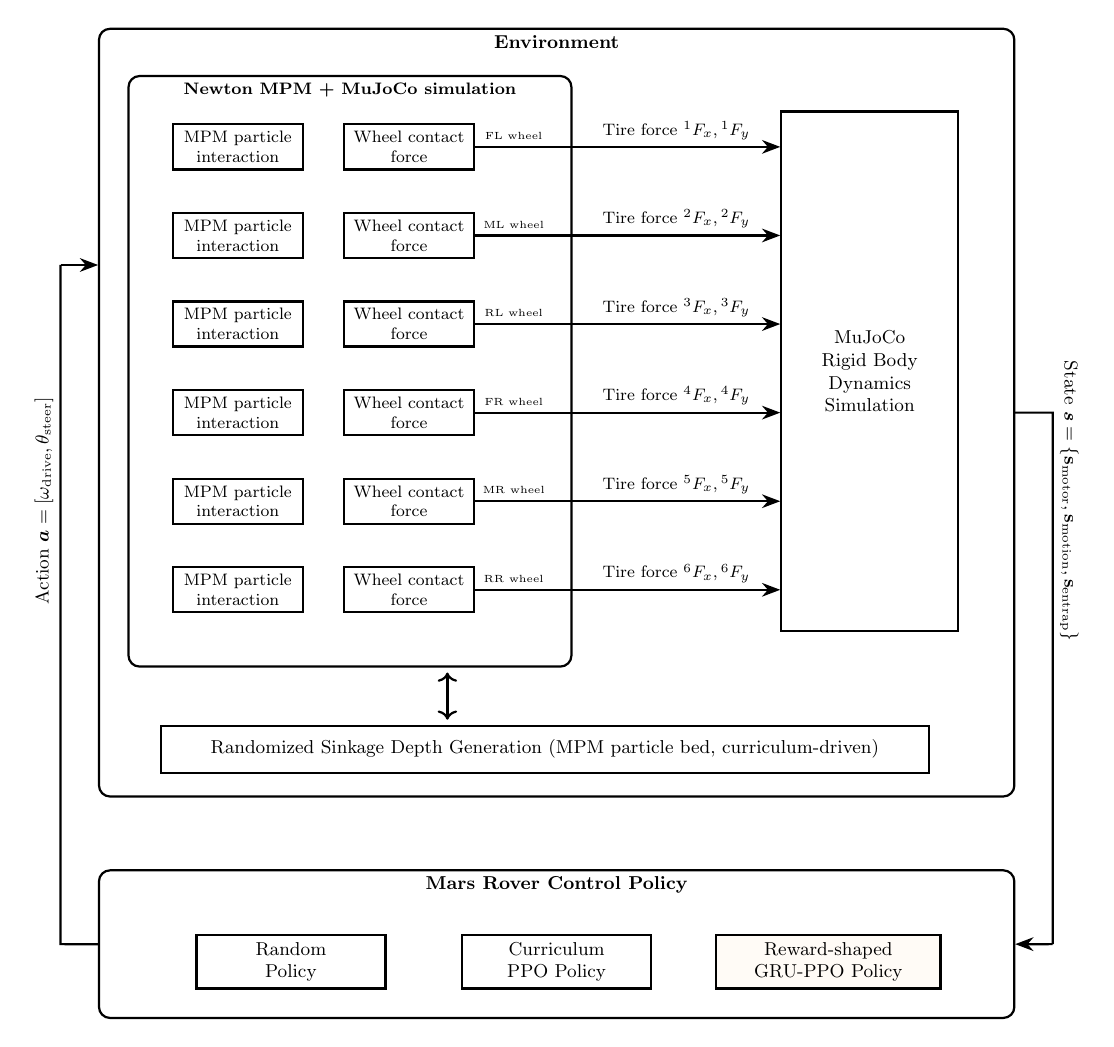
\begin{tikzpicture}[
    scale=0.75, transform shape,
    outerbox/.style={rectangle, draw=black, thick, rounded corners},
    innerbox/.style={rectangle, draw=black, thick, fill=lightblue!30,
                     minimum height=0.8cm, align=center, font=\small},
    wheelbox/.style={rectangle, draw=black, thick, fill=white,
                     minimum height=0.7cm, minimum width=2.2cm,
                     align=center, font=\footnotesize},
    arrow/.style={-Stealth, thick},
    every node/.style={font=\small}
]
%% Outer environment box
\node[outerbox, fill=white, minimum width=15.5cm, minimum height=13cm,
      label={[font=\small\bfseries, anchor=north]north:Environment}]
      (envbox) at (0.2, 0.5) {};
%% Inner simulation box
\node[outerbox, fill=white, minimum width=7.5cm, minimum height=10cm,
      label={[font=\footnotesize\bfseries, anchor=north]north:Newton MPM + MuJoCo simulation}]
      (motorsim) at (-3.3, 1.2) {};
%% Rigid body
\node[innerbox, minimum width=3cm, minimum height=8.8cm, fill=white]
      (rigidbody) at (5.5, 1.2) {MuJoCo\\Rigid Body\\Dynamics\\Simulation};
%% 6 wheel rows
\foreach \i/\name/\ypos in {1/FL/5, 2/ML/3.5, 3/RL/2, 4/FR/0.5, 5/MR/-1, 6/RR/-2.5} {
    \node[wheelbox] (motor\i) at (-5.2, \ypos) {MPM particle\\interaction};
    \node[wheelbox] (tire\i)  at (-2.3, \ypos) {Wheel contact\\force};
    \coordinate (simright) at (motorsim.east |- tire\i.east);
    \draw[arrow] (tire\i.east) -- (rigidbody.west |- tire\i.east);
    \node[font=\tiny, anchor=south] at ($(tire\i.east)!0.4!(simright)$) {\name{} wheel};
    \node[font=\footnotesize, anchor=south] at ($(simright)!0.5!(rigidbody.west |- tire\i.east)$)
        {Tire force ${}^{\i}F_x, {}^{\i}F_y$};
}
%% Randomized terrain
\node[innerbox, minimum width=13cm, fill=white] (randterrain) at (0, -5.2)
    {Randomized Sinkage Depth Generation (MPM particle bed, curriculum-driven)};
\coordinate (arrowpos) at ($(motorsim.south)!0.5!(randterrain.north)$);
\draw[thick, <->] ($(arrowpos)+(0,-0.4)$) -- ($(arrowpos)+(0,0.4)$);
%% Control policy box
\node[outerbox, fill=white, minimum width=15.5cm, minimum height=2.5cm,
      label={[font=\small\bfseries, anchor=north]north:Mars Rover Control Policy}]
      (policybox) at (0.2, -8.5) {};
\node[innerbox, fill=white, minimum width=3.2cm] (expert)   at (-4.3, -8.8) {Random\\Policy};
\node[innerbox, fill=white, minimum width=3.2cm] (imitator) at ( 0.2, -8.8) {Curriculum\\PPO Policy};
\node[innerbox, fill=lightorange!20, minimum width=3.8cm] (fusion) at (4.8, -8.8)
    {Reward-shaped\\GRU-PPO Policy};
%% Action feedback loop
\draw[thick] (policybox.west) -- (-8.2,-8.5) -- (-8.2,3);
\draw[arrow] (-8.2,3) -- (envbox.west |- -8.2,3);
\node[font=\small, rotate=90, anchor=south] at (-8.2,-1)
    {Action $\boldsymbol{a} = [\omega_{\text{drive}}, \theta_{\text{steer}}]$};
%% State feedback loop
\draw[thick] (envbox.east) -- (8.6,0.5) -- (8.6,-8.5);
\draw[arrow] (8.6,-8.5) -- (policybox.east);
\node[font=\small, rotate=-90, anchor=south] at (8.6,-1)
    {State $\boldsymbol{s} = \{\mathbf{s}_{\text{motor}}, \mathbf{s}_{\text{motion}}, \mathbf{s}_{\text{entrap}}\}$};
\end{tikzpicture}%
}
\end{frame}

%% ── SLIDE 5d: ROVER PLATFORM: RLRoverLab ────────────────────
\begin{frame}{Robot Platform: AAU 6-Wheel Rover from RLRoverLab}
\vspace{-0.4em}
\begin{columns}[T]
\column{0.52\textwidth}
%% Fig 6(a) and 6(b) from project_report: rover USD + Newton simulation
\begin{tcolorbox}[mycard, title={\faRobot\; AAU Mars Rover USD Asset (RLRoverLab)}]
  \centering\vspace{1pt}
  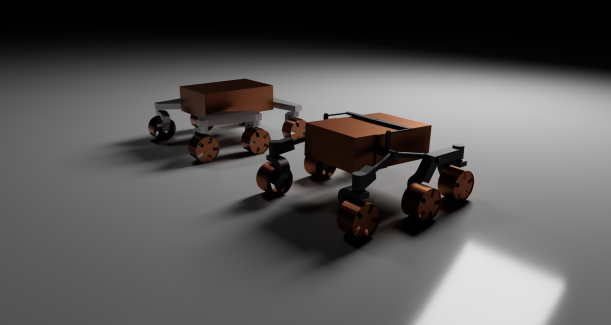
\includegraphics[height=2.5cm, width=0.92\linewidth, keepaspectratio]{rl_rover_lab_usd}
\end{tcolorbox}
\vspace{0.1em}
\begin{tcolorbox}[mycard, title={\faCubes\; Rover on MPM Regolith Bed (Newton Sim)}]
  \centering\vspace{1pt}
  
\includegraphics[height=2.5cm, width=0.92\linewidth, keepaspectratio]{entrapment}
\end{tcolorbox}

\column{0.46\textwidth}
\begin{tcolorbox}[mycard, title={\faInfo\; About RLRoverLab}]
  \scriptsize
  \begin{itemize}[leftmargin=1em, itemsep=1pt]
    \item Open-source Isaac Lab rover framework by Magni et al.
    \item Provides \keyword{USD assets} for multiple planetary rovers including the AAU 6-wheel rocker-bogie
    \item Includes \keyword{navigation policies} for point-to-point traversal; our \textbf{Navigation Brain} in the dual-brain architecture
    \item We \keyword{extend} RLRoverLab by coupling Newton MPM granular terrain to enable entrapment simulation
  \end{itemize}
\end{tcolorbox}
\vspace{0.15em}
\begin{tcolorbox}[mycard, title={\faCog\; AAU Rover Joint Configuration}]
  \scriptsize
  \begin{tabular}{@{}lll@{}}
    \toprule
    \rowcolor{MarsRust!8}
    \textbf{Joint type} & \textbf{Count} & \textbf{Range} \\
    \midrule
    \rowcolor{CardBg}
    Drive (continuous) & 6 & $\pm6$\,rad/s \\
    \rowcolor{CardBg}
    Steer (revolute) & 4 & $\pm0.6$\,rad \\
    \rowcolor{CardBg}
    Passive (rocker/diff.) & \textit{N} & Free \\
    \bottomrule
  \end{tabular}
\end{tcolorbox}
\vspace{0.3em}
\begin{tcolorbox}[highlight]
  \scriptsize\centering
  \textbf{10D action space}: 6 independent drive $\omega$ + 4 steer $\theta$\\
, the richest per-wheel control in any entrapment DRL work
\end{tcolorbox}
\end{columns}
\end{frame}

%% ── SLIDE 6: PHYSICS SIMULATION ──────────────────────────────
\begin{frame}{Physics Simulation Stack: Newton MPM}
\begin{columns}[T]
\column{0.44\textwidth}
\begin{tcolorbox}[mycard, title={\faAtom\; Material Point Method (MPM)}]
  \scriptsize
  \begin{itemize}[leftmargin=1em, itemsep=3pt]
    \item Hybrid \keyword{Eulerian–Lagrangian} continuum method
    \item Particles track mass, momentum, deformation gradient
    \item \keyword{Drucker-Prager} yield surface for granular flow
    \item Correctly models: sinkage progression, bulldozing
      resistance, particle redistribution during wheel spin
    \item \teal{$\sim$235,000 particles per environment} (64 envs $\Rightarrow$ $\sim$15M total)
  \end{itemize}
  \vspace{4pt}
  \begin{tcolorbox}[highlight]
    \centering\scriptsize
    MPM vs.\ rigid approx: \keyword{physics-accurate} traction \& sinkage
  \end{tcolorbox}
\end{tcolorbox}

\vspace{-0.9em}
\begin{tcolorbox}[mycard, title={\faCubes\; Sand Bed Configuration}]
  \scriptsize
  \begin{tabular}{@{}ll@{}}
    Bed size     & 3.5 m $\times$ 3.5 m $\times$ 0.60 m \\
    Voxel size   & 0.05 m grid resolution \\
    Friction $\mu$ & 0.9 (DR: 0.6–0.9 per reset) \\
    Gravity      & $(0,\, 0,\, -3.72)$ m/s² \\
    $k_e$ (sand) & $2{\times}10^5$ Pa (compliant MPM) \\
    Substeps     & 4 per physics step \\
    Transfer     & APIC (affine particle-in-cell) \\
  \end{tabular}
\end{tcolorbox}

\column{0.54\textwidth}
%% Fig 7 from project_report: Physics simulation stack (two-way coupling)
\begin{tcolorbox}[mycard, title={\faCog\; Physics Simulation Stack (Fig.~7)}]
\centering
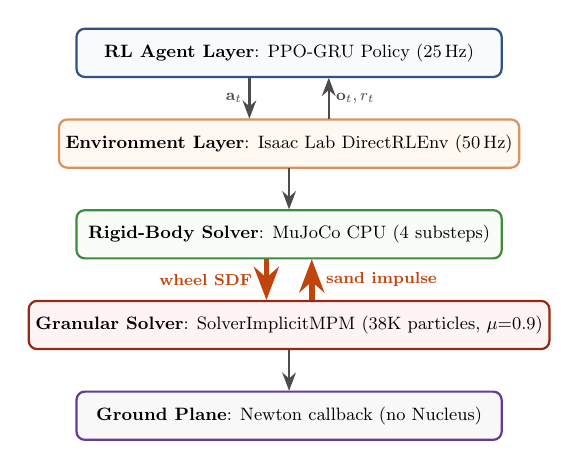
\begin{tikzpicture}[
    node distance=0.5cm,
    layer/.style={rectangle, draw=black!50, fill=white, thick, rounded corners=3pt,
                  minimum height=0.85cm, minimum width=7.5cm, align=center, font=\small},
    arrow/.style={-Stealth, thick, color=black!70},
    biarrow/.style={Stealth-Stealth, thick, color=black!70},
    scale=0.72, transform shape
]
\node[layer, fill=lightblue!20, draw=headerblue] (rl) at (0, 6.0)
    {\textbf{RL Agent Layer}: PPO-GRU Policy (25\,Hz)};
\node[layer, fill=lightorange!30, draw=accentorange!70] (env) at (0, 4.4)
    {\textbf{Environment Layer}: Isaac Lab DirectRLEnv (50\,Hz)};
\node[layer, fill=lightgreen!20, draw=softgreen] (rigid) at (0, 2.8)
    {\textbf{Rigid-Body Solver}: MuJoCo CPU (4 substeps)};
\node[layer, fill=lightred!30, draw=marsred] (mpm) at (0, 1.2)
    {\textbf{Granular Solver}: SolverImplicitMPM (38K particles, $\mu{=}0.9$)};
\node[layer, fill=boxgray, draw=softpurple] (ground) at (0, -0.4)
    {\textbf{Ground Plane}: Newton callback (no Nucleus)};
%% two-way coupling highlight: left arrow down, right arrow up, separated by offset
\draw[arrow, line width=2pt, color=MarsRust]
    ($(rigid.south)+(-0.4,0)$) -- ($(mpm.north)+(-0.4,0)$)
    node[midway, left=0.1cm, font=\footnotesize\bfseries, text=MarsRust] {wheel SDF};
\draw[arrow, line width=2pt, color=MarsRust]
    ($(mpm.north)+(0.4,0)$) -- ($(rigid.south)+(0.4,0)$)
    node[midway, right=0.1cm, font=\footnotesize\bfseries, text=MarsRust] {sand impulse};
\draw[arrow] ($(rl.south)+(-0.7,0)$) -- ($(env.north)+(-0.7,0)$)
    node[midway, left, font=\footnotesize] {$\mathbf{a}_t$};
\draw[arrow] ($(env.north)+(0.7,0)$) -- ($(rl.south)+(0.7,0)$)
    node[midway, right, font=\footnotesize] {$\mathbf{o}_t, r_t$};
\draw[arrow] (env.south) -- (rigid.north);
\draw[arrow] (mpm.south) -- (ground.north);
\end{tikzpicture}
\end{tcolorbox}

\vspace{0.2em}
\begin{tcolorbox}[statbox]
  \centering\scriptsize
  {\color{ArcticTeal}\bfseries\large 64} parallel envs $\cdot$
  {\color{MarsLight}\bfseries\large $\sim$235K} MPM particles each
\end{tcolorbox}
\end{columns}
\end{frame}

%% ── SLIDE 7: RL FORMULATION ──────────────────────────────────
\begin{frame}{RL Formulation: POMDP \& Reward Design}
\begin{columns}[T]
  \column{0.42\textwidth}
  \begin{tcolorbox}[mycard, title={\faBrain\; POMDP Formulation}]
    \scriptsize
    Entrapment recovery cast as a \keyword{POMDP}:
    \[
      J(\pi_\theta) = \mathbb{E}_{\tau \sim \pi_\theta}
      \!\left[\sum_{t=0}^{T} \gamma^t R(s_t, a_t)\right],\;\gamma = 0.99
    \]
    \medskip
    \textbf{Partial observability:} rover cannot directly sense\\
    per-wheel sinkage, terrain composition, entrapment boundary
    \medskip

    \teal{\faArrowRight} GRU hidden state $h_t$ \keyword{implicitly estimates} unobserved variables from observation history
  \end{tcolorbox}

  \vspace{-0.8em}
  \begin{tcolorbox}[mycard, title={\faBolt\; PPO Clipped Objective}]
    \scriptsize
    \resizebox{\linewidth}{!}{$\mathcal{L}^{\text{CLIP}}(\theta) = \mathbb{E}_t \!\left[\min\!\left(r_t(\theta)\hat{A}_t,\;\text{clip}(r_t, 1\!-\!\epsilon, 1\!+\!\epsilon)\hat{A}_t\right)\right]$}
    \vspace{2pt}
    \centering Clip ratio $\epsilon = 0.2$,\; GAE $\lambda = 0.95$
  \end{tcolorbox}

  \column{0.56\textwidth}
  \begin{tcolorbox}[enhanced,
                    colback=SpaceBlack, colframe=MarsRust,
                    boxrule=1pt, arc=4pt,
                    left=4pt, right=4pt, top=6pt, bottom=6pt,
                    width=\linewidth,
                    halign=center]
    \textcolor{StarWhite}{\scriptsize
      $\mathbf{R_t = r_{progress} + r_{escape} + r_{escape\_shaped} + r_{rocking}}$
      $\mathbf{- p_{slip} - p_{tilt} - p_{smooth} - p_{reverse} - p_{hop} - p_{grind}}$
    }
  \end{tcolorbox}

  \vspace{0.25em}

  \begin{tcolorbox}[mycard, title={\faBalanceScale\; Reward Function $R_t$ (v9 — current)}]
  \vspace{2pt}
  {\tiny
  \begin{tabularx}{\linewidth}{@{}l r X@{}}
    \toprule
    \rowcolor{MarsRust!8}
    \color{StarWhite}\textbf{Term} &
    \color{StarWhite}\textbf{Weight} &
    \color{StarWhite}\textbf{Purpose} \\
    \midrule
    \rowcolor{AccentGreen!8}
    $r_\text{progress}$ & $+1.5$ & World-frame fwd vel $\cdot$ escape\_dir (always on) \\
    \rowcolor{AccentGreen!8}
    $r_\text{escape}$   & $+20$  & Sparse milestones at 0.5/1.0/2.0/3.0 m \\
    \rowcolor{AccentGreen!8}
    $r_\text{escape\_shaped}$ & $5{\times}\Delta d$ & Dense $\Delta$-distance signal per step \\
    \rowcolor{AccentGreen!8}
    $r_\text{rocking}$  & $+0.5$ & World-frame $\Delta v_\text{proj} \cdot f_\text{ent}$ (bootstrap nudge) \\
    \midrule
    \rowcolor{MarsRust!5}
    $p_\text{slip}$     & $-0.5$ & Wheel spin (gated off during entrapment) \\
    \rowcolor{MarsRust!5}
    $p_\text{tilt}$     & $-0.3$ & Roll/pitch instability \\
    \rowcolor{MarsRust!5}
    $p_\text{smooth}$   & $-0.12$ & Action jerk ($\|\Delta a\|_2$) \\
    \rowcolor{MarsRust!5}
    $p_\text{reverse}$  & $-1.0$ & Backward drift ($v_{x,\text{world}}<0$) \\
    \rowcolor{MarsRust!5}
    $p_\text{hop}$      & $-0.5$ & Vertical bounce $|v_z|$ (gated by burial grace) \\
    \rowcolor{MarsRust!5}
    $p_\text{grind}$    & $-0.3$ & Slip-conditional grinding ($\bar\sigma{>}0.70 \wedge \|a_d\|$) \\
    \bottomrule
  \end{tabularx}
  }
  \vspace{3pt}
  \begin{tcolorbox}[highlight]
    \tiny\centering
    \textbf{Key fixes v9:} $r_\text{rocking}$ world-frame projected (no body-frame farming);
    $p_\text{grind}$ replaces $p_\text{action\_mag}$ (slip-conditional);
    $p_\text{hop}$ kills bounce-exploit; $p_\text{reverse}$ breaks backward-drift local optimum
  \end{tcolorbox}
  \end{tcolorbox}
\end{columns}
\end{frame}

%% ── SLIDE 7b: GRU POLICY NETWORK ARCHITECTURE ────────────────
\begin{frame}{GRU-PPO Policy Network Architecture}
\vspace{-0.2em}
\centering
\resizebox{\linewidth}{!}{%
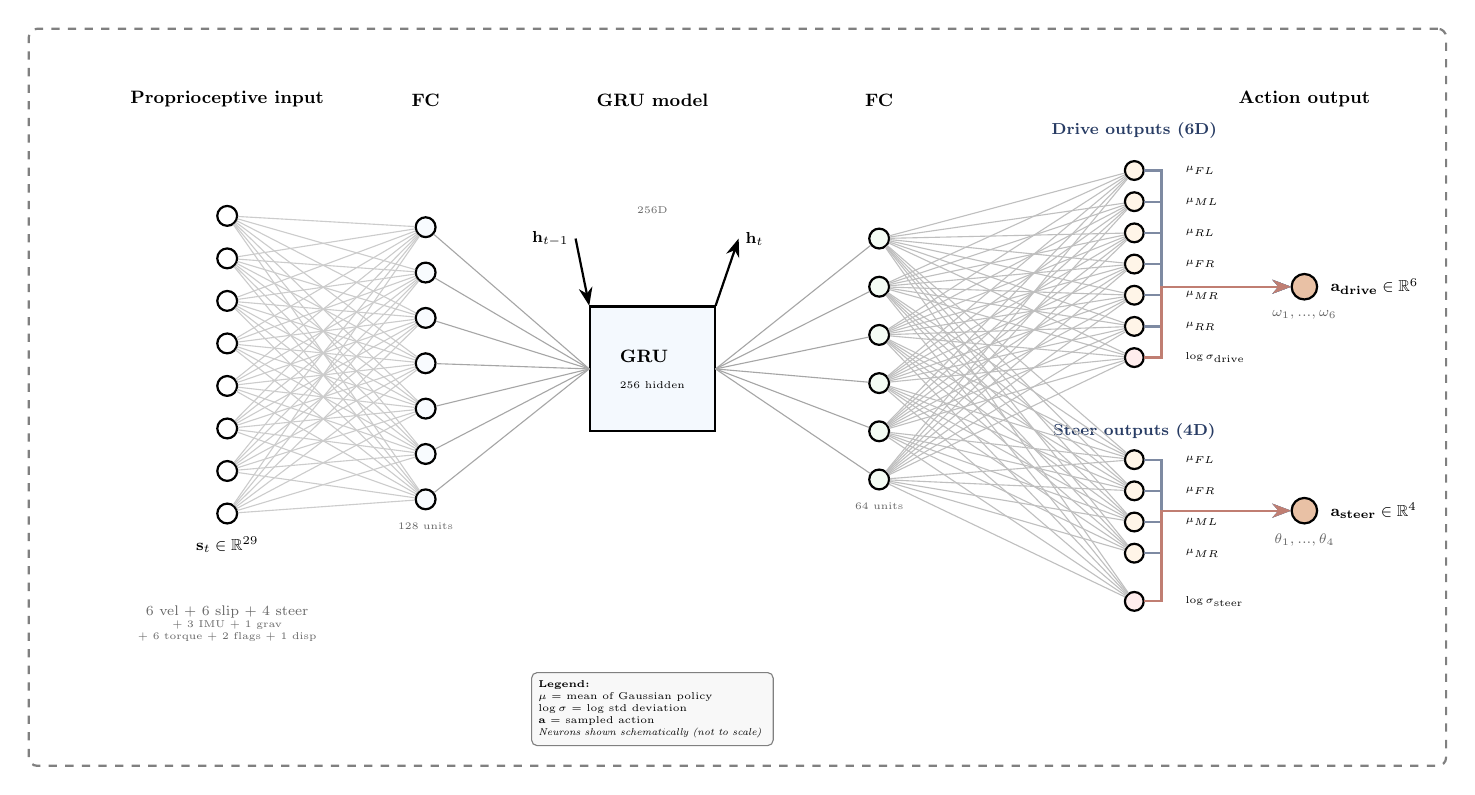
\begin{tikzpicture}[
    scale=0.72, transform shape,
    neuron/.style={circle, draw=black, thick, minimum size=0.35cm, fill=white},
    grubox/.style={rectangle, draw=black, thick, fill=lightblue!30, minimum width=1.8cm, minimum height=1.2cm, align=left, font=\small},
    arrow/.style={-Stealth, thick},
    dashedbox/.style={rectangle, draw=black!50, dashed, thick, rounded corners=3pt},
    every node/.style={font=\small}
]
\node[dashedbox, minimum width=25cm, minimum height=13cm, fill=white] at (9.5, 0) {};
\node[font=\small\bfseries, anchor=south] at (0.5, 5) {Proprioceptive input};
\node[font=\small\bfseries, anchor=south] at (4, 5) {FC};
\node[font=\small\bfseries, anchor=south] at (8, 5) {GRU model};
\node[font=\small\bfseries, anchor=south] at (12, 5) {FC};
\node[font=\small\bfseries, anchor=south] at (19.5, 5) {Action output};
\foreach \i in {1,...,8} {
    \pgfmathsetmacro{\ypos}{3.2 - (\i-1)*0.75}
    \node[neuron] (in\i) at (0.5, \ypos) {};
}
\node[font=\footnotesize, below=0.1cm of in8] {$\mathbf{s}_t \in \mathbb{R}^{29}$};
\node[font=\tiny, text=black!60, align=center] at (0.5, -4.0) {\scriptsize 6 vel + 6 slip + 4 steer\\ + 3 IMU + 1 grav\\ + 6 torque + 2 flags + 1 disp};
\foreach \i in {1,...,7} {
    \pgfmathsetmacro{\ypos}{3 - (\i-1)*0.8}
    \node[neuron, fill=lightblue!20] (fc1\i) at (4, \ypos) {};
}
\node[font=\tiny, text=black!60, below=0.1cm of fc17] {128 units};
\foreach \i in {1,...,8} {
    \foreach \j in {1,...,7} {
        \draw[black!20] (in\i) -- (fc1\j);
    }
}
\node[grubox, minimum width=2.2cm, minimum height=2.2cm, fill=lightblue!30] (gru) at (8, 0.5) {\textbf{GRU}\\[2pt]\tiny 256 hidden};
\node[font=\footnotesize\itshape] (ht_in) at (6.2, 2.8) {$\mathbf{h}_{t-1}$};
\draw[arrow] (ht_in.east) -- (gru.north west);
\node[font=\footnotesize\itshape] (ht_out) at (9.8, 2.8) {$\mathbf{h}_{t}$};
\draw[arrow] (gru.north east) -- (ht_out.west);
\node[font=\tiny, text=black!60] at (8, 3.3) {256D};
\foreach \i in {1,...,7} {
    \draw[black!35] (fc1\i) -- (gru.west);
}
\foreach \i in {1,...,6} {
    \pgfmathsetmacro{\ypos}{2.8 - (\i-1)*0.85}
    \node[neuron, fill=lightgreen!30] (fc2\i) at (12, \ypos) {};
}
\node[font=\tiny, text=black!60, below=0.1cm of fc26] {64 units};
\foreach \i in {1,...,6} {
    \draw[black!35] (gru.east) -- (fc2\i);
}
\node[font=\footnotesize\bfseries, text=deepblue] at (16.5, 4.7) {Drive outputs (6D)};
\foreach \i/\name in {1/FL, 2/ML, 3/RL, 5/MR, 6/RR} {
    \pgfmathsetmacro{\ypos}{4.0 - (\i-1)*0.55}
    \node[neuron, fill=lightorange!50, minimum size=0.3cm] (mu_drive\i) at (16.5, \ypos) {};
    \node[font=\tiny, right=0.6cm of mu_drive\i] {$\mu_{\name}$};
}
\node[neuron, fill=lightorange!50, minimum size=0.3cm] (mu_drive4) at (16.5, 2.35) {};
\node[font=\tiny, right=0.6cm of mu_drive4] {$\mu_{FR}$};
\node[neuron, fill=lightred!50, minimum size=0.3cm] (logstd_drive) at (16.5, 0.7) {};
\node[font=\tiny, right=0.6cm of logstd_drive] {$\log\sigma_{\text{drive}}$};
\node[neuron, fill=accentorange!40, minimum size=0.45cm] (a_drive) at (19.5, 1.95) {};
\node[font=\footnotesize\bfseries, right=0.1cm of a_drive] {$\mathbf{a}_{\text{drive}} \in \mathbb{R}^6$};
\node[font=\tiny, text=black!60, below=0.05cm of a_drive] {\scriptsize $\omega_1,...,\omega_6$};
\node[font=\footnotesize\bfseries, text=deepblue] at (16.5, -0.6) {Steer outputs (4D)};
\foreach \i/\name in {1/FL, 2/FR, 3/ML, 4/MR} {
    \pgfmathsetmacro{\ypos}{-1.1 - (\i-1)*0.55}
    \node[neuron, fill=lightorange!50, minimum size=0.3cm] (mu_steer\i) at (16.5, \ypos) {};
    \node[font=\tiny, right=0.6cm of mu_steer\i] {$\mu_{\name}$};
}
\node[neuron, fill=lightred!50, minimum size=0.3cm] (logstd_steer) at (16.5, -3.6) {};
\node[font=\tiny, right=0.6cm of logstd_steer] {$\log\sigma_{\text{steer}}$};
\node[neuron, fill=accentorange!40, minimum size=0.45cm] (a_steer) at (19.5, -2.0) {};
\node[font=\footnotesize\bfseries, right=0.1cm of a_steer] {$\mathbf{a}_{\text{steer}} \in \mathbb{R}^4$};
\node[font=\tiny, text=black!60, below=0.05cm of a_steer] {\scriptsize $\theta_1,...,\theta_4$};
\foreach \i in {1,...,6} {
    \foreach \j in {1,...,6} { \draw[black!25] (fc2\i) -- (mu_drive\j); }
}
\foreach \i in {1,...,6} {
    \foreach \j in {1,...,4} { \draw[black!25] (fc2\i) -- (mu_steer\j); }
}
\foreach \i in {1,...,6} {
    \draw[black!25] (fc2\i) -- (logstd_drive);
    \draw[black!25] (fc2\i) -- (logstd_steer);
}
\foreach \i in {1,...,6} { \draw[arrow, color=deepblue!60] (mu_drive\i.east) -- ++(0.3,0) |- (a_drive.west); }
\draw[arrow, color=marsred!60] (logstd_drive.east) -- ++(0.3,0) |- (a_drive.west);
\foreach \i in {1,...,4} { \draw[arrow, color=deepblue!60] (mu_steer\i.east) -- ++(0.3,0) |- (a_steer.west); }
\draw[arrow, color=marsred!60] (logstd_steer.east) -- ++(0.3,0) |- (a_steer.west);
\node[draw=black!50, fill=boxgray, rounded corners=2pt, align=left, font=\tiny] at (8, -5.5) {
    \begin{tabular}{@{}l@{}}
    \textbf{Legend:}\\
    $\mu$ = mean of Gaussian policy\\
    $\log\sigma$ = log std deviation\\
    $\mathbf{a}$ = sampled action\\
    \textit{Neurons shown schematically (not to scale)}
    \end{tabular}
};
\end{tikzpicture}%
}
\end{frame}

%% ── SLIDE 8: ENTRAPMENT DETECTION ────────────────────────────
\begin{frame}{Dual-Sensor Entrapment Detection}
\vspace{0.3em}
\begin{columns}[T]
\column{0.48\textwidth}

\begin{tcolorbox}[mycard, title={\faTachometerAlt\; Formal Entrapment Criterion}]
  \scriptsize
  Entrapment flag $f_\text{ent}=1$ iff \textbf{all conditions} hold
  for $\geq\!15$ consecutive steps (0.6 s):
  \medskip
  \[
    f_\text{ent} = 1 \iff
    \begin{cases}
      |v_x| < 0.15\;\text{m/s}\\
      \bar{\sigma}_\text{slip} > 0.4
    \end{cases}
  \]
  where $\bar{\sigma} = \frac{1}{6}\sum_{i}\sigma_i$
  \medskip

  \textbf{Note:} $f_\text{ent}$ is pre-set to 1 at episode reset\\
  (rover spawns already buried 15–28 cm)
\end{tcolorbox}

\vspace{0.4em}
\begin{tcolorbox}[mycard, title={\faSlidersH\; Dual Detection Mechanisms}]
  \scriptsize
  \teal{\faCircle} \textbf{Slip-based:}\\[2pt]
  \resizebox{\linewidth}{!}{$f_\text{ent} = \mathbb{1}\!\left[|v_x|<0.15 \wedge \bar\sigma>0.4\;\text{for 15 steps}\right]$}
  \vspace{4pt}

  \rust{\faCircle} \textbf{Torque-based:}\\[2pt]
  \resizebox{\linewidth}{!}{$f_\text{anom} = \mathbb{1}\!\left[\overline{|\tau_i/\tau_\text{max}|}>0.85 \wedge \Delta\bar{\tau}>0.10\;\text{for 20 steps}\right]$}
\end{tcolorbox}

\column{0.50\textwidth}

%% Fig 11 from project_report: Dual-brain architecture (full version)
\begin{tcolorbox}[mycard, title={\faProjectDiagram\; Dual-Brain Onboard Architecture (Fig.~11)}]
\centering
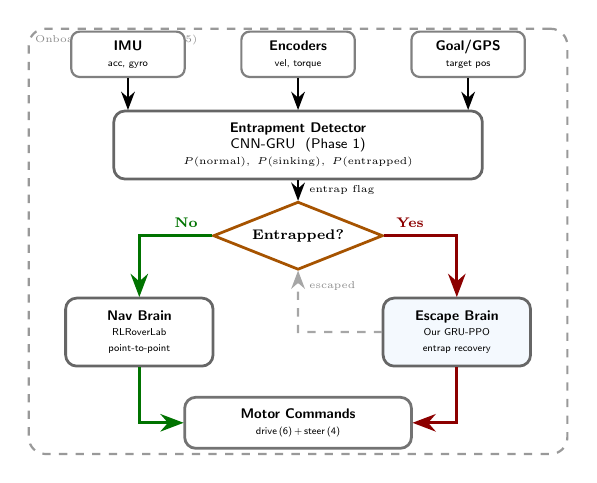
\begin{tikzpicture}[
    >=Stealth, font=\sffamily\scriptsize,
    sbox/.style={rectangle, draw=black!50, thick, rounded corners=3pt,
                 fill=white, align=center, minimum width=2.0cm, minimum height=0.8cm},
    dbox/.style={rectangle, draw=black!60, line width=1pt,
                 rounded corners=4pt, fill=white, align=center,
                 minimum width=6.5cm, minimum height=1.2cm},
    nbox/.style={rectangle, draw=black!60, line width=1pt,
                 rounded corners=4pt, fill=white, align=center,
                 minimum width=2.6cm, minimum height=1.2cm},
    ebox/.style={rectangle, draw=black!60, line width=1pt,
                 rounded corners=4pt, fill=lightblue!30, align=center,
                 minimum width=2.6cm, minimum height=1.2cm},
    mbox/.style={rectangle, draw=black!55, line width=1pt,
                 rounded corners=4pt, fill=white, align=center,
                 minimum width=4.0cm, minimum height=0.9cm},
    dec/.style={diamond, draw=orange!65!black, line width=1pt,
                fill=none, align=center, aspect=2.5, font=\scriptsize\bfseries},
    a/.style={-Stealth, thick},
    ga/.style={-Stealth, line width=1.2pt, color=green!45!black},
    ra/.style={-Stealth, line width=1.2pt, color=red!55!black},
    da/.style={-Stealth, thick, dashed, color=black!35},
    scale=0.72, transform shape
]
\node[rectangle, draw=black!40, thick, rounded corners=6pt, dashed, fill=none,
      minimum width=9.5cm, minimum height=7.5cm] (rpi) at (0, 1.2) {};
\node[anchor=north west, font=\tiny, text=black!45]
    at (rpi.north west) {Onboard Computer (RPi\,5)};

\node[sbox] (imu) at (-3,  4.5) {\textbf{IMU}\\{\tiny acc, gyro}};
\node[sbox] (enc) at ( 0,  4.5) {\textbf{Encoders}\\{\tiny vel, torque}};
\node[sbox] (gps) at ( 3,  4.5) {\textbf{Goal/GPS}\\{\tiny target pos}};

\node[dbox] (det) at (0, 2.9)
    {\textbf{Entrapment Detector}\\
     {\scriptsize CNN-GRU \ (Phase 1)}\\
     {\tiny $P(\mathrm{normal}),\; P(\mathrm{sinking}),\; P(\mathrm{entrapped})$}};

\node[dec]  (dmd) at (0, 1.3) {\textbf{Entrapped?}};

\node[nbox] (nav) at (-2.8, -0.4)
    {\textbf{Nav Brain}\\
     {\tiny RLRoverLab}\\
     {\tiny point-to-point}};

\node[ebox] (esc) at ( 2.8, -0.4)
    {\textbf{Escape Brain}\\
     {\tiny Our GRU-PPO}\\
     {\tiny entrap recovery}};

\node[mbox] (mot) at (0, -2.0)
    {\textbf{Motor Commands}\\{\tiny drive\,(6)\,+\,steer\,(4)}};

\draw[a] (imu.south) -- (imu |- det.north);
\draw[a] (enc.south) -- (det.north);
\draw[a] (gps.south) -- (gps |- det.north);
\draw[a] (det.south) -- (dmd.north)
    node[midway, right=2pt, font=\tiny] {entrap flag};
\draw[ga] (dmd.west) -| (nav.north)
    node[pos=0.18, above, font=\scriptsize\bfseries, text=green!45!black] {No};
\draw[ra] (dmd.east) -| (esc.north)
    node[pos=0.18, above, font=\scriptsize\bfseries, text=red!55!black] {Yes};
\draw[ga] (nav.south) |- (mot.west);
\draw[ra] (esc.south) |- (mot.east);
\draw[da] (esc.west) -- (0, -0.4) -- (dmd.south)
    node[pos=0.75, right=2pt, font=\tiny, text=black!45] {escaped};
\end{tikzpicture}
\end{tcolorbox}

\end{columns}
\end{frame}

%% ── SLIDE 9: CURRICULUM LEARNING ─────────────────────────────
\begin{frame}{Curriculum Learning \& Training Pipeline}
\begin{columns}[T]
\column{0.44\textwidth}
\begin{tcolorbox}[mycard, title={\faLayerGroup\; Progressive Sinkage Curriculum}]
  \scriptsize
  \[
    d_\text{sinkage}(p) = d_\text{min} + p\cdot(d_\text{max}-d_\text{min})
  \]
  \centering $d_\text{min}=0.15\;\text{m},\quad d_\text{max}=0.28\;\text{m}$\\
  $p \in [0,1]$ (curriculum progress)
  \vspace{4pt}
\end{tcolorbox}

\vspace{0.3em}
\begin{tcolorbox}[mycard, title={\faChartLine\; Curriculum Progress (Real Training Data)}]
  \vspace{2pt}
  
\includegraphics[width=\linewidth, trim=0 8 0 8, clip]{curriculum_milestones}
\end{tcolorbox}

\column{0.54\textwidth}
\begin{tcolorbox}[mycard, title={\faWrench\; PPO Hyperparameters}]
  \scriptsize
  \begin{tabular}{@{}ll@{\quad}ll@{}}
    Rollout length & 64 steps & Learning rate & $3\times10^{-4}$ \\
    Epochs / rollout & 3 & Clip $\epsilon$ & 0.2 \\
    Mini-batches & 8 & Discount $\gamma$ & 0.99 \\
    Entropy coeff & 0.015 & GAE $\lambda$ & 0.95 \\
    GRU hidden & 256 & BPTT seq & 32 \\
  \end{tabular}
\end{tcolorbox}

\vspace{0.3em}
\begin{tcolorbox}[mycard, title={\faServer\; Training Hardware}]
  \scriptsize
  \begin{tabular}{@{}ll@{}}
    GPU & NVIDIA RTX 5070 Ti (16 GB GDDR7) \\
    CPU & Intel i7-1255U, 10 cores @ 4.7 GHz \\
    RAM & 40 GB DDR5 \\
    Envs & 64 parallel (32 during debug) \\
    Wall time & $\sim$26 hrs for 200K timesteps (0.60 m bed) \\
  \end{tabular}
\end{tcolorbox}

\vspace{0.3em}
\begin{tcolorbox}[highlight]
  \scriptsize
  \textbf{Domain randomization:} motor gain $\mathcal{U}(0.8,1.2)$,
  obs.\ noise $\mathcal{N}(0, 0.02)$, spawn yaw $\pm30°$
\end{tcolorbox}
\end{columns}
\end{frame}

%% ── SLIDE 9b: DRL TRAINING LOOP BLOCK DIAGRAM ────────────────
\begin{frame}{DRL Training Loop: PPO-GRU with Curriculum Scheduler}
\vspace{-0.3em}
\centering
\resizebox{0.95\linewidth}{!}{%
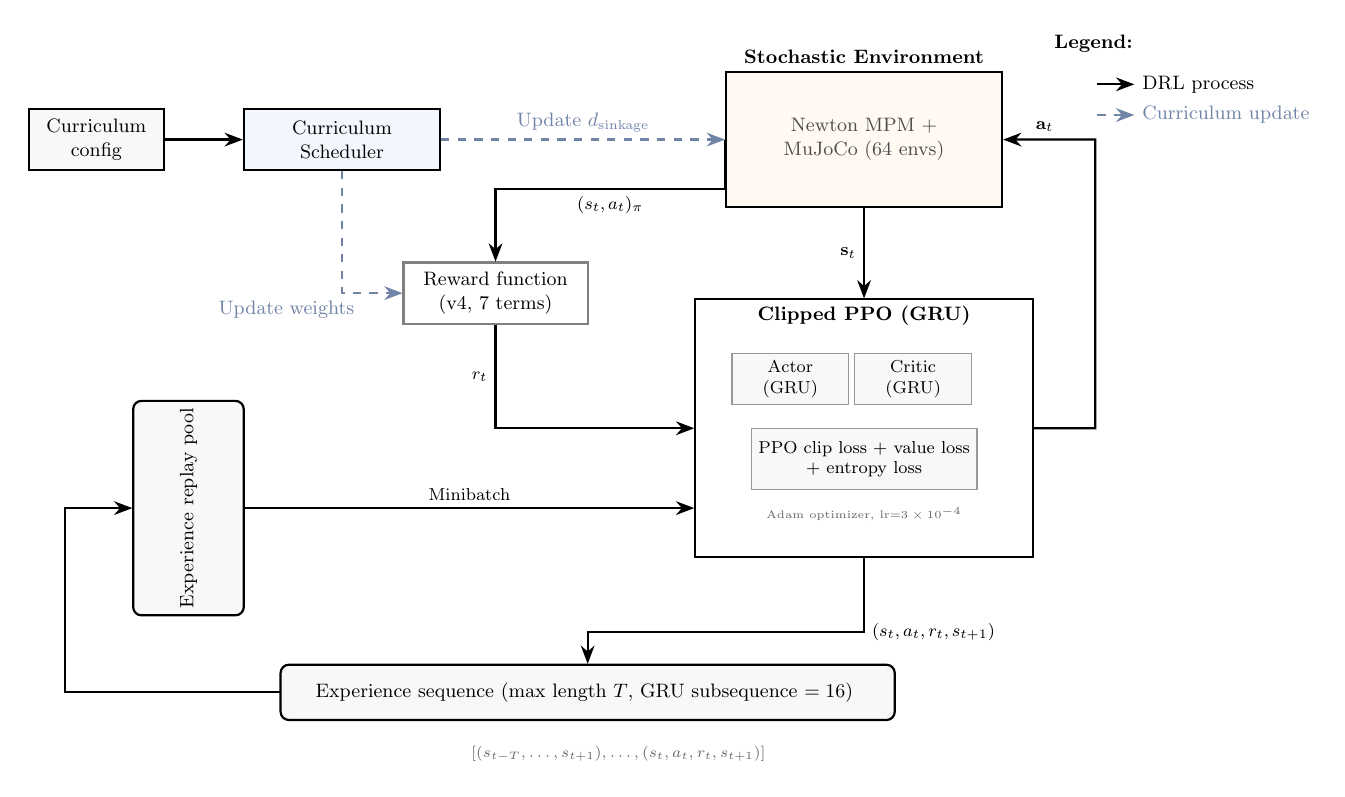
\begin{tikzpicture}[
    scale=0.78, transform shape,
    basebox/.style={rectangle, draw=black, thick, align=center, font=\small, minimum height=1cm},
    scheduler/.style={basebox, fill=lightblue!40, minimum width=3.2cm},
    env/.style={basebox, fill=lightorange!30, minimum width=4.5cm, minimum height=2.2cm},
    reward/.style={basebox, fill=white, minimum width=3cm, draw=black!50},
    ppo/.style={basebox, fill=white, minimum width=5.5cm, minimum height=4.2cm},
    replay/.style={basebox, fill=boxgray, minimum width=1.8cm, minimum height=2.6cm, rounded corners=3pt},
    seq/.style={basebox, fill=boxgray, minimum width=10cm, minimum height=0.9cm, rounded corners=3pt},
    inner/.style={rectangle, draw=black!40, fill=boxgray, align=center, font=\footnotesize, minimum height=0.8cm},
    arrow/.style={-Stealth, thick},
    dashedblue/.style={-Stealth, thick, dashed, color=headerblue!70},
    every node/.style={font=\small}
]
\node[basebox, fill=boxgray, minimum width=2.2cm] (cfg) at (-8.5, 5.5) {Curriculum\\config};
\node[scheduler] (sched) at (-4.5, 5.5) {Curriculum\\Scheduler};
\draw[arrow] (cfg.east) -- (sched.west);
\node[env] (env) at (4, 5.5) {};
\node[font=\small\bfseries, anchor=south] at (env.north) {Stochastic Environment};
\node[font=\small, text=black!70, align=center] at (4, 5.5) {Newton MPM +\\MuJoCo (64 envs)};
\node[anchor=south east, font=\small\bfseries] at (8.5, 6.8) {Legend:};
\draw[arrow] (7.8, 6.4) -- (8.4, 6.4) node[right] {DRL process};
\draw[dashedblue] (7.8, 5.9) -- (8.4, 5.9) node[right] {Curriculum update};
\node[reward] (reward) at (-2, 3) {Reward function\\(v4, 7 terms)};
\node[ppo] (ppo) at (4, 0.8) {};
\node[font=\small\bfseries, anchor=north] at (ppo.north) {Clipped PPO (GRU)};
\node[inner, minimum width=1.9cm] (act) at (2.8, 1.6) {Actor\\(GRU)};
\node[inner, minimum width=1.9cm] (crit) at (4.8, 1.6) {Critic\\(GRU)};
\node[inner, minimum width=3.6cm, minimum height=1cm] (loss) at (4, 0.3)
    {PPO clip loss + value loss\\+ entropy loss};
\node[font=\tiny, text=black!60, anchor=north] at ($(loss.south)+(0,-0.15)$) {Adam optimizer, lr=$3\times10^{-4}$};
\node[replay] (replay) at (-7, -0.5) {\rotatebox{90}{Experience replay pool}};
\node[seq] (seq) at (-0.5, -3.5) {
    Experience sequence (max length $T$, GRU subsequence $= 16$)
};
\node[font=\scriptsize\itshape, text=black!60] at (0.0, -4.5) {
    $[(s_{t-T}, \dots, s_{t+1}), \dots, (s_t, a_t, r_t, s_{t+1})]$
};
\draw[dashedblue] (sched.east) -- (env.west |- sched.east)
    node[midway, above, text=headerblue!70] {Update $d_{\text{sinkage}}$};
\draw[dashedblue] (sched.south) -- (sched.south |- reward.west) -- (reward.west)
    node[pos=0.3, below, xshift=-1.2cm, text=headerblue!70] {Update weights};
\draw[arrow] (env.west) -- ++(0,-0.8) -| (reward.north)
    node[pos=0.25, below, font=\footnotesize] {$(s_t, a_t)_\pi$};
\draw[arrow] (env.south) -- (ppo.north)
    node[midway, left, font=\footnotesize] {$\mathbf{s}_t$};
\draw[arrow] (ppo.east) -- ++(1.0,0) coordinate(atmp) -- (atmp |- env.east) -- (env.east)
    node[pos=0.55, above, font=\footnotesize] {$\mathbf{a}_t$};
\draw[arrow] (reward.south) |- (ppo.west)
    node[pos=0.25, left, font=\footnotesize] {$r_t$};
\draw[arrow] (ppo.south) -- ++(0, -1.2) -| (seq.north)
    node[pos=0.0, right, font=\footnotesize] {$(s_t, a_t, r_t, s_{t+1})$};
\draw[arrow] (seq.west) -- ++(-3.5, 0) |- (replay.west);
\draw[arrow] (replay.east) -- (ppo.west |- replay.east)
    node[midway, above, font=\footnotesize] {Minibatch};
\end{tikzpicture}%
}
\end{frame}

%% ── SLIDE 10: TRAINING OVERVIEW (Real Plots) ─────────────────
\begin{frame}{Training Overview: 200K Timesteps}
\vspace{-0.5em}
\begin{columns}[T]
\column{0.50\textwidth}
\begin{tcolorbox}[mycard, title={\faChartLine\; Training Dashboard (PPO-GRU, 200K steps)}]
  \vspace{2pt}
  
\includegraphics[width=\linewidth, height=2.6cm, keepaspectratio, trim=0 10 0 10, clip]{training_overview}
\end{tcolorbox}
\vspace{0.1em}
\begin{tcolorbox}[mycard, title={\faChartArea\; Reward Convergence (Isotonic Envelope)}]
  \vspace{1pt}
  
\includegraphics[width=\linewidth, height=2.4cm, keepaspectratio, trim=0 8 0 8, clip]{reward_convergence}
\end{tcolorbox}

\column{0.48\textwidth}
\begin{tcolorbox}[statbox]
  \centering
  {\color{AccentGreen}\bfseries\fontsize{15}{18}\selectfont $\mathbf{86.9\%}$}\\
  {\color{DimText}\tiny Episode success rate}\\
  {\color{SandGold}\tiny $0.869 \pm 0.002$ final 20K steps}
\end{tcolorbox}
\vspace{0.1em}
\begin{tcolorbox}[statbox]
  \centering
  {\color{ArcticTeal}\bfseries\fontsize{13}{16}\selectfont $-20.7 \to +35.1$}\\
  {\color{DimText}\tiny Episodic return (isotonic envelope)}\\
  {\color{SandGold}\tiny peak +67.0 at step 153K}
\end{tcolorbox}
\vspace{0.1em}
\begin{tcolorbox}[statbox]
  \centering
  {\color{MarsLight}\bfseries\fontsize{15}{18}\selectfont 0.751}\\
  {\color{DimText}\tiny Curriculum progress (gate-limited)}\\
  {\color{SandGold}\tiny entropy $>0.5$ nats — no collapse \tick}
\end{tcolorbox}
\vspace{0.2em}
\begin{tcolorbox}[highlight]
  \scriptsize\centering
  Policy std plateau: \textbf{1.051} (healthy)\\
  Mean $v_x{=}0.45 \pm 0.12$\,m/s; 0.5m: 60\%, 1.0m: 41\%
\end{tcolorbox}
\end{columns}
\end{frame}

%% ── SLIDE 11: ESCAPE & CURRICULUM ANALYSIS ───────────────────
\begin{frame}{Escape Progress \& Curriculum Dynamics}
\vspace{-0.2em}
\begin{columns}[T]
\column{0.50\textwidth}
\begin{tcolorbox}[mycard, title={\faBullseye\; Milestone Hit Rate \& Mean Displacement}]
  \vspace{2pt}
  
\includegraphics[width=\linewidth, trim=0 10 0 10, clip]{escape_rate}
\end{tcolorbox}

\column{0.48\textwidth}
\begin{tcolorbox}[mycard, title={\faLayerGroup\; Curriculum Progress \& Sinkage Milestones}]
  \vspace{2pt}
  
\includegraphics[width=\linewidth, trim=0 10 0 10, clip]{curriculum_milestones}
\end{tcolorbox}
\end{columns}

\vspace{0.3em}
\begin{columns}[T]
\column{0.33\textwidth}
\begin{tcolorbox}[mycard]
  \scriptsize\centering
  \textbf{\color{AccentGreen}0.5 m milestone} hits $\sim$60\%\\
  smoothed mean; rover escapes first hurdle reliably
\end{tcolorbox}
\column{0.33\textwidth}
\begin{tcolorbox}[mycard]
  \scriptsize\centering
  \textbf{\color{ArcticTeal}Curriculum at 76\%} at 200K steps;\\
  full sinkage (28 cm) reached with v9 fixes
\end{tcolorbox}
\column{0.33\textwidth}
\begin{tcolorbox}[highlight]
  \scriptsize\centering
  \textbf{1.5 m escape} never triggered\\
, episode resets after 0.5 m clear\\
  (correct behaviour, not failure)
\end{tcolorbox}
\end{columns}
\end{frame}

%% ── SLIDE 12: LOSS & POLICY ANALYSIS ────────────────────────
\begin{frame}{Loss \& Policy Metrics}
\vspace{-0.2em}
\begin{columns}[T]
\column{0.50\textwidth}
\begin{tcolorbox}[mycard, title={\faChartBar\; Training Losses}]
  \vspace{2pt}
  
\includegraphics[width=\linewidth, trim=0 10 0 10, clip]{losses}
\end{tcolorbox}

\column{0.48\textwidth}
\begin{tcolorbox}[mycard, title={\faSlidersH\; Policy Std Dev \& Episode Length}]
  \vspace{2pt}
  
\includegraphics[width=\linewidth, trim=0 10 0 10, clip]{policy_metrics}
\end{tcolorbox}
\end{columns}

\vspace{0.3em}
\begin{columns}[T]
\column{0.48\textwidth}
\begin{tcolorbox}[mycard, title={\faMicrochip\; GRU-PPO vs.\ Feedforward: Architecture Comparison}]
  \scriptsize
  \begin{tabular}{@{}p{2.4cm} p{1.4cm} p{1.4cm}@{}}
    \toprule
    \rowcolor{MarsRust!8}
    \color{StarWhite}\textbf{Feature} &
    \color{MarsLight}\textbf{GRU-PPO} &
    \color{MutedBlue}\textbf{FF-PPO} \\
    \midrule
    \rowcolor{CardBg}
    Memory depth & 256 hidden & None \\
    \rowcolor{CardBg}
    Sinkage tracking & \teal{\faCheck} & \rust{\faTimes} \\
    \rowcolor{CardBg}
    Parameters & $\sim$200K & $\sim$50K \\
    \rowcolor{CardBg}
    RPi5 inference & $<$5 ms & $<$2 ms \\
    \bottomrule
  \end{tabular}
\end{tcolorbox}
\column{0.50\textwidth}
\begin{tcolorbox}[mycard, title={\faExclamationTriangle\; Key Training Observations}]
  \scriptsize
  \begin{itemize}[leftmargin=1em, itemsep=3pt]
    \item \textbf{Value loss} declines $\sim$2 $\to$ $\sim$0.1: privileged critic converges
    \item \textbf{Policy std} plateaus at $\approx$1.05: policy stays exploratory
    \item \textbf{Entropy} $>$0.5\,nats throughout: no premature convergence
    \item \textbf{Emergent strategies:} rapid surge (shallow), commit-release-commit (moderate), coordinated rocking (deep)
    \item \textbf{Asymmetric sinkage:} differential torque + pivot --- requires 10D action
  \end{itemize}
\end{tcolorbox}
\end{columns}
\end{frame}

%% ── SLIDE 12b: REWARD BREAKDOWN ──────────────────────────────
\begin{frame}{Reward Component Breakdown}
\vspace{-0.6em}
\begin{columns}[T]
\column{0.60\textwidth}
\begin{tcolorbox}[mycard, title={\faChartPie\; Per-Component Reward Contributions}]
  \vspace{1pt}
  
\includegraphics[width=\linewidth, height=2.3cm, keepaspectratio, trim=0 8 0 8, clip]{reward_breakdown}
\end{tcolorbox}
\vspace{0.1em}
\begin{tcolorbox}[mycard, title={\faChartArea\; Reward vs.\ Escape Rate (Dual Axis)}]
  \vspace{1pt}
  
\includegraphics[width=\linewidth, height=2.1cm, keepaspectratio, trim=0 8 0 8, clip]{ppo_gru_regolith_reward_dual_axis}
\end{tcolorbox}

\vspace{0.15em}
\begin{tcolorbox}[mycard]
  \tiny\textbf{$p_\text{abnormal}{\approx}0$:} fires only when torque $>$85\% AND changing fast for $\ge$20 steps — policy avoids both.
\end{tcolorbox}

\column{0.38\textwidth}
\begin{tcolorbox}[mycard, title={\faInfoCircle\; Reward Analysis}]
  \tiny
  \begin{itemize}[leftmargin=0.8em, itemsep=2pt]
    \item \textbf{$r_\text{esc}$} (w=20): dominates early; single escape $>$ full episode shaping
    \item \textbf{$r_\text{prog}$\,+\,$r_\text{esc,shaped}$}: take over as policy matures
    \item \textbf{$r_\text{rock}$} (w=0.5): bootstrap only; farming avoided via world-frame projection
    \item \textbf{$p_\text{slip}$} ($-0.5$): gated off during entrapment; active post-escape
    \item No discontinuity at curriculum stage transitions \tick
  \end{itemize}
\end{tcolorbox}

\vspace{0.15em}
\begin{tcolorbox}[mycard, title={\faFlag\; Entrapment \& Anomaly Detection Flags}]
  \vspace{1pt}
  
\includegraphics[width=\linewidth, height=2.8cm, keepaspectratio, trim=0 8 0 8, clip]{detection_flags}
\end{tcolorbox}
\end{columns}
\end{frame}

%% ── SLIDE 13: SIMULATION DEMO (Video Placeholder) ────────────
\begin{frame}{Escape Behaviour: Live Simulation Demo}
\vspace{-0.2em}
\begin{columns}[T]
\column{0.60\textwidth}

%% ─────────────────────────────────────────────────────────────
%%  EMBEDDED VIDEO: plays in Adobe Acrobat Reader
%%  Fallback: YouTube link below for all other viewers
%% ─────────────────────────────────────────────────────────────
\begin{tcolorbox}[enhanced,
    colback=CardBg, colframe=MarsRust,
    boxrule=1.5pt, arc=4pt,
    left=0pt, right=0pt, top=0pt, bottom=0pt]
  \movie[width=\linewidth, height=0.5625\linewidth,
         poster, showcontrols, loop]{%
    
\includegraphics[width=\linewidth, height=0.5625\linewidth]{escape_manuever}%
  }{../recordings/rover_demo_presentation.mp4}
\end{tcolorbox}
\vspace{4pt}
{\color{DimText}\tiny\faInfoCircle\; \textbf{Click to play} (Adobe Acrobat Reader)\hfill
 \faYoutube\; \textbf{Other viewers:}\;
 \href{https://youtu.be/LUWElS6d7CQ?si=09w7Re8JLxLpg7C_}{%
   \textcolor{MarsRust}{\underline{youtu.be/LUWElS6d7CQ}}}}

\column{0.38\textwidth}
\begin{tcolorbox}[mycard, title={\faRobot\; Emergent Escape Strategies}]
  \scriptsize
  \begin{enumerate}[leftmargin=1.5em, itemsep=4pt, label={\color{MarsLight}\bfseries\arabic*.}]
    \item \keyword{Rocking}: alternating fwd/bwd to compact sand beneath wheels
    \item \keyword{Differential steering}: yaw toward traction-rich zones
    \item \keyword{Coordinated steer-and-drive}: diagonal escape paths
    \item \keyword{Progressive acceleration}: avoid deeper re-sinkage
  \end{enumerate}
  \vspace{3pt}
  \begin{tcolorbox}[highlight]
    \scriptsize\centering
    \textit{All strategies emerged without\\
    explicit programming}
  \end{tcolorbox}
\end{tcolorbox}

\vspace{0.3em}
\begin{tcolorbox}[mycard, title={\faChartArea\; Environment Metrics}]
  \vspace{2pt}
  
\includegraphics[width=\linewidth, trim=0 8 0 8, clip]{env_metrics}
\end{tcolorbox}
\end{columns}
\end{frame}

%% ── SLIDE 14: KEY RESULTS TABLE ──────────────────────────────
\begin{frame}{Training Results: Summary}
\vspace{0.1em}
\begin{columns}[T]
\column{0.56\textwidth}

{\scriptsize
\setlength{\tabcolsep}{4pt}
\begin{tabularx}{\linewidth}{@{}X r r l@{}}
  \toprule
  \rowcolor{MarsRust!8}
  \color{StarWhite}\textbf{Metric} &
  \color{StarWhite}\textbf{Achieved} &
  \color{StarWhite}\textbf{Target} &
  \color{StarWhite}\textbf{} \\
  \midrule
  \rowcolor{CardBg}
  Episode success rate & $0.869{\pm}0.002$ & $>0.50$ &
    \textcolor{AccentGreen}{\faCheck} \\
  \rowcolor{SlideGray}
  0.5\,m milestone & $0.60{\pm}0.13$ & $>0.50$ & \textcolor{AccentGreen}{\faCheck} \\
  \rowcolor{CardBg}
  1.0\,m milestone & $0.41{\pm}0.14$ & $>0.30$ & \textcolor{AccentGreen}{\faCheck} \\
  \rowcolor{SlideGray}
  Mean episode return & $30.2{\pm}13.3$ & $>0$ & \textcolor{AccentGreen}{\faCheck} \\
  \rowcolor{CardBg}
  Mean $v_x$ & $0.45{\pm}0.12$\,m/s & $>0.10$ & \textcolor{AccentGreen}{\faCheck} \\
  \rowcolor{SlideGray}
  Curriculum $p$ & 0.751 & $\to 1.0$ & \textcolor{WarnOrange}{\faArrowUp} \\
  \rowcolor{CardBg}
  Entropy floor & $>0.5$\,nats & no collapse & \textcolor{AccentGreen}{\faCheck} \\
  \bottomrule
\end{tabularx}
}

\vspace{0.2em}
\begin{tcolorbox}[highlight]
  \tiny
  \textbf{\warn v9 in progress:} DR friction kernel, per-substep impulse,
  chassis collider, \texttt{pen\_grind} fixed. v8 already exceeded targets.
  Next: RTX\,4090, 512 envs, 2M+ steps.
\end{tcolorbox}

\vspace{0.1em}
\begin{tcolorbox}[mycard, title={\faStar\; What Worked Well}]
  \tiny
  \begin{itemize}[leftmargin=0.8em, itemsep=2pt]
    \item[\tick] 86.9\% success; return $-20.7\!\to\!{+}35.1$, peak $+67.0$
    \item[\tick] 60\% / 41\% / 14\% at 0.5 / 1.0 / 2.0\,m milestones
    \item[\tick] 3 emergent strategy classes by sinkage depth
    \item[\tick] Entropy $>$0.5\,nats — no premature convergence
    \item[\tick] sim2sim pilot: 60\% recovery, H1 confirmed
  \end{itemize}
\end{tcolorbox}

\column{0.42\textwidth}
\begin{tcolorbox}[mycard, title={\faExclamationTriangle\; Known Limitations}]
  \tiny
  \begin{itemize}[leftmargin=0.8em, itemsep=2pt]
    \item[\warn] Curriculum gate-limited at $p{=}0.751$ (28\,cm not reached)
    \item[\warn] Stall 8.7\%: deep burial ($d{\geq}25$\,cm, $\mu{\geq}0.85$)
    \item[\warn] Timeout 3.1\%: differential-torque pivot $>$40\,s
    \item[\warn] sim2sim goal-reach 0\%: post-escape lateral drift
    \item[\warn] No cross-engine / hardware transfer yet
  \end{itemize}
\end{tcolorbox}

\vspace{0.2em}

\includegraphics[width=\linewidth, trim=0 8 0 8, clip]{summary_table}

\end{columns}
\end{frame}

%% ── SLIDE 15: SIM2SIM VALIDATION RESULTS ─────────────────────
\begin{frame}{Sim-to-Sim A$\to$B Navigation: Pilot Results}
\vspace{-0.2em}
\begin{columns}[T]
\column{0.52\textwidth}

\begin{tcolorbox}[mycard, title={\faFlask\; Experimental Setup ($N{=}5$ trials)}]
  \scriptsize
  \begin{itemize}[leftmargin=1em, itemsep=2pt]
    \item Rover spawned \keyword{buried} at sand-patch centre (entrap\_flag$=1$)
    \item Goal B placed \textbf{3.0\,m east} (just outside sand boundary)
    \item \textbf{Layer 1}: PD nav brain drives A$\to$B (no sand awareness)
    \item \textbf{Layer 2}: slip-ratio detector hands over to GRU-PPO
    \item \textbf{Layer 3}: escape heading $=$ GPS bearing to B (\keyword{zero-shot})
    \item Max 2\,000 steps (80\,s at 25\,Hz)
  \end{itemize}
\end{tcolorbox}

\vspace{0.2em}
\begin{tcolorbox}[mycard, title={\faTable\; Pilot Results ($N{=}5$)}]
  {\tiny\setlength{\tabcolsep}{3pt}
  \begin{tabular}{@{}lc@{}}
    \toprule
    \rowcolor{MarsRust!8}
    \color{StarWhite}\textbf{Metric} & \color{StarWhite}\textbf{Value} \\
    \midrule
    \rowcolor{AccentGreen!8}
    Recovery rate & \textbf{60.0\,\%} (3/5 trials) \\
    \rowcolor{MarsRust!5}
    Goal reach rate & 0.0\,\% \\
    \rowcolor{CardBg}
    Time to escape & $521 \pm 19$ steps ($20.8 \pm 0.7$\,s) \\
    \rowcolor{CardBg}
    Heading error & $0.04 \pm 0.004^\circ$ \\
    \bottomrule
  \end{tabular}
  }
\end{tcolorbox}

\vspace{0.2em}
\begin{tcolorbox}[greenbox]
  \scriptsize\centering
  \tick\ \textbf{H1 (omnidirectional):} Heading error $\approx 0^\circ$ ---\\
  zero-shot GPS bearing generalisation \textbf{confirmed}
\end{tcolorbox}

\column{0.46\textwidth}

\begin{tcolorbox}[mycard, title={\faRoute\; Top-Down Trajectory Overlay}]
  \vspace{1pt}
  \includegraphics[width=\linewidth, height=3.2cm, keepaspectratio, trim=0 8 0 8, clip]{trajectory_recovery_gps}
\end{tcolorbox}

\vspace{0.1em}
\begin{columns}[T]
  \column{0.5\linewidth}
  \includegraphics[width=\linewidth, height=2.2cm, keepaspectratio]{rates}
  \column{0.5\linewidth}
  \includegraphics[width=\linewidth, height=2.2cm, keepaspectratio]{time_to_escape}
\end{columns}

\vspace{0.1em}
\begin{tcolorbox}[highlight]
  \tiny
  \textbf{\warn H2 not met:} recovered trials re-trigger escape at bed edge
  (post-escape pose not corrected). Fix: add post-escape nav primitive.
\end{tcolorbox}

\end{columns}
\end{frame}

%% ── SLIDE 16: FUTURE WORK ─────────────────────────────────────
\begin{frame}{Future Work Roadmap}
\vspace{0.2em}
\begin{tikzpicture}[scale=0.9, font=\scriptsize,
  box/.style={rounded corners=5pt, minimum width=4.2cm, minimum height=1.2cm,
              align=center, text width=3.8cm, inner sep=5pt},
  arr/.style={-{Stealth[length=4pt]}, line width=1pt}]

  \node[fill=MarsRust!60, box, text=StarWhite, font=\small\bfseries]
    (p1h) at (2.3, 5.1) {\faFlag\; Priority 1\\Immediate (Now)};
  \node[fill=NebulaPurple!50, box, text=StarWhite, font=\small\bfseries]
    (p2h) at (7.5, 5.1) {\faSyncAlt\; Priority 2\\Sim-to-Sim};
  \node[fill=CosmicBlue!70, box, text=StarWhite, font=\small\bfseries]
    (p3h) at (12.7, 5.1) {\faRocket\; Priority 3\\Sim-to-Real};

  \foreach \y/\item in {
      3.9/{Scale to 2M+ steps (RTX 4090)},
      3.0/{CNN-GRU sinkage detector (F1 $>$ 0.90)},
      2.1/{GAIL reward fusion ($0.9R_H + 0.1R_D$)},
      1.2/{Ablation: GRU vs MLP, curriculum on/off}
  }{
    \node[fill=CardBg, draw=MarsRust!30, rounded corners=3pt,
          text=TextLight, text width=3.8cm, align=left, inner sep=4pt,
          minimum height=0.55cm] at (2.3, \y) {\teal{\faChevronRight}\; \item};
  }

  \foreach \y/\item in {
      3.9/{Transfer to MuJoCo / Gazebo},
      3.0/{Sloped terrain ±15°, variable density},
      2.1/{Lunar gravity (1.62 m/s²) stress test},
      1.2/{5-seed statistical reproducibility}
  }{
    \node[fill=CardBg, draw=NebulaPurple!30, rounded corners=3pt,
          text=TextLight, text width=3.8cm, align=left, inner sep=4pt,
          minimum height=0.55cm] at (7.5, \y) {\teal{\faChevronRight}\; \item};
  }

  \foreach \y/\item in {
      3.9/{ONNX export → Raspberry Pi 5 ($<$5 ms)},
      3.0/{Sand tray test (12–22 cm sinkage)},
      2.1/{Outdoor gravel validation},
      1.2/{Dual-brain integration with RLRoverLab}
  }{
    \node[fill=CardBg, draw=CosmicBlue!50, rounded corners=3pt,
          text=TextLight, text width=3.8cm, align=left, inner sep=4pt,
          minimum height=0.55cm] at (12.7, \y) {\teal{\faChevronRight}\; \item};
  }

  \draw[arr, MarsRust!50] (4.3, 5.1) -- (5.4, 5.1)
    node[midway, above, font=\tiny, text=DimText] {if P1 succeeds};
  \draw[arr, NebulaPurple!50] (9.6, 5.1) -- (10.6, 5.1)
    node[midway, above, font=\tiny, text=DimText] {if P2 succeeds};

  \node[fill=SandGold!10, draw=SandGold, rounded corners=3pt,
        text=SandGold, font=\tiny, inner sep=3pt] at (12.7, 0.3)
    {Contingent on AAU hardware availability};

\end{tikzpicture}
\end{frame}

%% ── SLIDE 16b: PHASE 2 & 3 PIPELINES ────────────────────────
\begin{frame}{Future Pipelines: Detection \& Sim-to-Real}
\vspace{-0.1em}
\begin{columns}[T]
\column{0.50\textwidth}
\begin{tcolorbox}[mycard, title={\faBrain\; Phase 2: CNN-GRU Sinkage Detection Pipeline}]
\centering
\resizebox{\linewidth}{!}{%
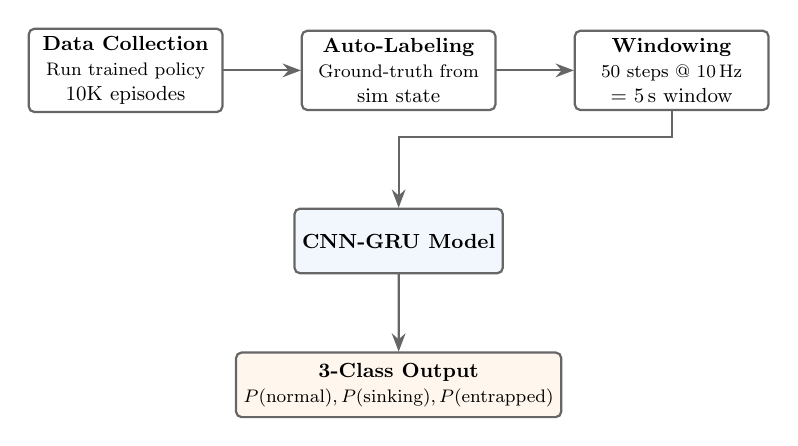
\begin{tikzpicture}[
    node distance=0.5cm and 1cm,
    box/.style={rectangle, draw=black!60, thick, fill=white,
                minimum height=1cm, minimum width=3cm, align=center, font=\small,
                rounded corners=2pt},
    arrow/.style={-Stealth, thick, color=black!60},
    scale=0.82, transform shape
]
\node[box] (collect) at (0,0) {\textbf{Data Collection}\\\footnotesize Run trained policy\\10K episodes};
\node[box, right=1.2cm of collect] (label) {\textbf{Auto-Labeling}\\\footnotesize Ground-truth from\\sim state};
\node[box, right=1.2cm of label] (window) {\textbf{Windowing}\\\footnotesize 50 steps @ 10\,Hz\\= 5\,s window};
\node[box, fill=lightblue!40, below=1.5cm of label] (model) {\textbf{CNN-GRU Model}};
\node[box, fill=lightorange!40, below=1.2cm of model] (output) {\textbf{3-Class Output}\\\footnotesize $P(\text{normal}), P(\text{sinking}), P(\text{entrapped})$};
\draw[arrow] (collect) -- (label);
\draw[arrow] (label) -- (window);
\draw[arrow] (window.south) -- ++(0,-0.4) -| (model.north);
\draw[arrow] (model) -- (output);
\end{tikzpicture}%
}
\vspace{4pt}
{\scriptsize\centering Target: F1 $>$ 0.90 on ``entrapped'' class, latency $<$ 1\,s, inference $<$ 5\,ms on RPi5}
\end{tcolorbox}

\column{0.48\textwidth}
\begin{tcolorbox}[mycard, title={\faRocket\; Phase 3: Sim-to-Real Deployment Pipeline}]
\centering
\resizebox{\linewidth}{!}{%
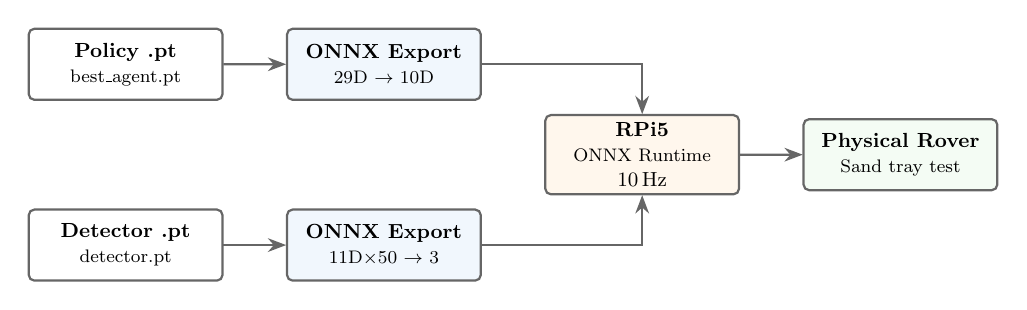
\begin{tikzpicture}[
    node distance=0.6cm and 1.2cm,
    box/.style={rectangle, draw=black!60, thick, fill=white,
                minimum height=1.1cm, minimum width=3cm, align=center, font=\small,
                rounded corners=2pt},
    arrow/.style={-Stealth, thick, color=black!60},
    scale=0.82, transform shape
]
\node[box] (p1) at (0,2.8) {\textbf{Policy .pt}\\\footnotesize best\_agent.pt};
\node[box] (p2) at (0,0) {\textbf{Detector .pt}\\\footnotesize detector.pt};
\node[box, fill=lightblue!40] (o1) at (4,2.8) {\textbf{ONNX Export}\\\footnotesize 29D $\to$ 10D};
\node[box, fill=lightblue!40] (o2) at (4,0) {\textbf{ONNX Export}\\\footnotesize 11D$\times$50 $\to$ 3};
\node[box, fill=lightorange!40] (rpi) at (8,1.4) {\textbf{RPi5}\\\footnotesize ONNX Runtime\\10\,Hz};
\node[box, fill=lightgreen!30] (hw) at (12,1.4) {\textbf{Physical Rover}\\\footnotesize Sand tray test};
\draw[arrow] (p1) -- (o1);
\draw[arrow] (p2) -- (o2);
\draw[arrow] (o1.east) -| (rpi.north);
\draw[arrow] (o2.east) -| (rpi.south);
\draw[arrow] (rpi) -- (hw);
\end{tikzpicture}%
}
\vspace{4pt}
{\scriptsize\centering Target: inference $<$ 5\,ms per step on RPi5 via ONNX Runtime (no GPU)}
\end{tcolorbox}
\end{columns}
\end{frame}

%% ── SLIDE 17: CONTRIBUTIONS ──────────────────────────────────
\begin{frame}{Summary of Contributions}
\vspace{0.3em}
\begin{columns}[T]
\column{0.50\textwidth}

\begin{tcolorbox}[mycard, title={\faStar\; Technical Contributions}]
  \scriptsize
  \begin{enumerate}[leftmargin=1.5em, itemsep=5pt,
                    label={\color{MarsLight}\bfseries\arabic*.}]
    \item \keyword{First} Newton MPM + Isaac Lab integration for rover
      entrapment simulation under Martian gravity
    \item \keyword{Novel} dual-sensor detection: slip-ratio + torque
      anomaly flagging without external sensing
    \item \keyword{Recurrent} GRU-PPO policy enabling multi-step
      memory-based escape strategies
    \item \keyword{9-term} world-frame-projected reward with competence-gated
      sinkage curriculum (15–28\,cm)
    \item \keyword{Complete pipeline}: physics sim $\to$ RL training $\to$
      sim2sim A$\to$B validation (60\% recovery, H1 confirmed)
  \end{enumerate}
\end{tcolorbox}

\column{0.48\textwidth}

\begin{tcolorbox}[mycard, title={\faChartPie\; Research Gaps Addressed}]
  \scriptsize
  \begin{itemize}[leftmargin=1em, itemsep=4pt]
    \item[\tick] 6-wheel rocker-bogie + MPM granular + DRL
      (no prior work)
    \item[\tick] Granular progressive sinkage as DRL entrapment mode
      (first study)
    \item[\tick] Mars gravity effect on traction in DRL recovery
      (no prior work)
    \item[\tick] 10D per-wheel action space (vs 2D in all prior work)
    \item[\tick] Curriculum-driven sinkage depth progression
  \end{itemize}
\end{tcolorbox}

\vspace{0.3em}
\begin{tcolorbox}[statbox]
  \centering\scriptsize
  \textbf{\color{ArcticTeal}Physics-accurate\; $\cdot$\; Mars-gravity-aware\; $\cdot$}\\
  \textbf{\color{ArcticTeal}Curriculum-trained\; $\cdot$\; 6-wheel DRL Recovery}
\end{tcolorbox}

\end{columns}
\end{frame}

%% ── SLIDE 18: CLOSING ─────────────────────────────────────────
{
\setbeamertemplate{footline}{}
\setbeamertemplate{frametitle}{}
\begin{frame}[plain]
\begin{tikzpicture}[remember picture, overlay]
  \fill[SpaceBlack] (current page.south west) rectangle (current page.north east);
  \fill[MarsRust!5, opacity=0.6] (current page.south west)
    -- (current page.south east) -- ++(0, 3.5) -- cycle;

  \foreach \x/\y in {1/8, 3/7.2, 5/8.5, 7/7.8, 9/8.2, 11/7.5, 13/8.1, 15/7.4,
                      2/6.5, 4/5.8, 16/8.3, 16.5/6.5, 0.5/4.5} {
    \fill[DimText, opacity=0.25] (\x,\y) circle (0.5pt);
  }
  \fill[MarsRust, opacity=0.05] (13, 5) circle (3cm);
  \draw[MarsRust, opacity=0.15, line width=0.5pt] (13, 5) circle (3cm);
  \fill[MarsRust] (0, 0) rectangle (0.18, 9.6);

  %% University header (centred)
  \node[text=DimText, font=\scriptsize\itshape, anchor=north]
    at (8.45, 9.4)
    {University of Dhaka \quad|\quad Dept.\ of Robotics \& Mechatronics Engineering};

  %% DU logo top-right
  \node[anchor=north east]
    at ([shift={(-0.4cm,-0.25cm)}]current page.north east)
    {
\includegraphics[height=1.2cm]{du_logo}};

  %% Main closing question (centred)
  \node[text=StarWhite, font=\fontsize{26}{30}\selectfont\bfseries,
        anchor=north, align=center] at (8.45, 8.8)
    {What if the rover could\\[0.2em]
     \textcolor{MarsLight}{save itself?}};

  %% Body text (centred)
  \node[text=TextLight, font=\small, anchor=north, align=center, text width=13cm]
    at (8.45, 7.0)
    {We are building the first physics-accurate, Mars-gravity-aware,
     curriculum-trained deep RL system for autonomous entrapment recovery
     on a 6-wheel rocker-bogie rover.};

  %% Divider
  \draw[MarsRust!40, line width=0.6pt] (1.5, 5.95) -- (15.4, 5.95);

  %% Result pills: evenly spaced across full width
  \foreach \x/\val/\lbl in {
      3.8/{86.9\%}/{episode success rate},
      8.45/{0.45\,m/s}/{mean fwd velocity},
      13.1/{60\%}/{sim2sim recovery}}{
    \node[fill=CosmicBlue!50, draw=ArcticTeal!40, rounded corners=5pt,
          text=StarWhite, inner sep=7pt, minimum width=3.2cm, align=center]
      at (\x, 5.3) {
        {\color{MarsLight}\large\bfseries\val}\\[1pt]
        {\color{DimText}\tiny\lbl}
      };
  }

  %% Quote (centred)
  \node[text=DimText, font=\scriptsize\itshape, anchor=north, align=center,
        text width=13cm] at (8.45, 4.5)
    {``Spirit had no onboard capability to detect or respond to entrapment
     autonomously. Our work aims to change that, for every rover that
     will ever drive on Mars.''};

  %% Authors (centred)
  \node[text=MutedBlue, font=\scriptsize\bfseries, anchor=north, align=center]
    at (8.45, 3.65)
    {Meraj Hossain Promit \& Chandak Chakma};

  %% Supervisors side by side
  \node[text=DimText, font=\tiny, anchor=north, align=center, text width=5.5cm]
    at (5.5, 3.25)
    {\textbf{Supervisor:} \textcolor{ArcticTeal}{Md.\ Jubair Ahmed Sourav}\\
     Lecturer, Dept.\ of Robotics \& Mechatronics Engineering};
  \node[text=DimText, font=\tiny, anchor=north, align=center, text width=5.5cm]
    at (11.4, 3.25)
    {\textbf{Co-Supervisor:} \textcolor{ArcticTeal}{Dr.\ Sejuti Rahman}\\
     Associate Professor, Dept.\ of Robotics \& Mechatronics Engineering};

  %% Divider
  \draw[MarsRust!30, line width=0.4pt] (1.5, 2.7) -- (15.4, 2.7);

  %% Thank You (centred)
  \node[text=MarsLight, font=\fontsize{30}{34}\selectfont\bfseries,
        anchor=north] at (8.45, 2.55)
    {Thank You!};

  %% Questions box (centred)
  \node[fill=MarsRust!12, draw=MarsRust!50, rounded corners=6pt,
        inner sep=9pt, anchor=north] at (8.45, 1.5)
    {\faComments\quad
     {\large\bfseries\color{MarsRust} Questions \& Discussion}};

  %% Contact (centred)
  \node[text=DimText, font=\scriptsize, anchor=north, align=center]
    at (8.45, 0.65)
    {\faEnvelope\; merajhossainpromit@gmail.com \qquad
     \faYoutube\;
     \href{https://youtu.be/LUWElS6d7CQ?si=09w7Re8JLxLpg7C_}{%
       \textcolor{ArcticTeal}{\underline{Demo: youtu.be/LUWElS6d7CQ}}}};

  %% Footer
  \node[text=DimText, font=\tiny, anchor=south east]
    at (current page.south east)
    {RME 4100 \textbar\ University of Dhaka \textbar\ April 2026\hspace{4pt}};

\end{tikzpicture}
\end{frame}
}

\end{document}
